% !TeX root = ../main.tex

\chapter{龙芯安卓图形栈详细设计与实现}
本章将详细介绍在现有龙芯硬件平台下,图形系统的三个重要组成部分:内核图形驱动模块,安卓gralloc模块和硬件混合渲染(HWC)模块。内核驱动模块负责对接用户态驱动
和GPU固件之间的联系。而gralloc模块是根据龙芯硬件驱动向安卓上层libui库提供服务,硬件混合渲染(HWC)模块为安卓中进行窗口(Layer)合成和显示的HAL模块。
随后说明了如何构建龙芯显卡的OpenGL ES支持以及定制部分安卓系统镜像。

\section{GPU驱动内核模块的实现}
现代操作系统对硬件资源的管理存在两种典型的设计模式\cite{马超2015linux}:
1.直接访问模式​(如 MS-DOS):允许用户程序绕过内核直接操作硬件设备,通过物理地址空间或专用 I/O 端口实现低级控制
2.抽象隔离模式​(如 Linux):内核通过硬件抽象层(HAL)屏蔽物理设备细节,所有硬件操作必须通过标准化的系统调用\cite{刘大同2016vxworks}(如 open(), ioctl())发起,内核负责资源调度和安全审查。
驱动程序就是操作系统内核和硬件沟通的桥梁,准确来说就是内核的一部分。

\subsection{IOCTL命令码设计}
\label{sec:IOCTL命令码设计}
在内核驱动程序中,除了基本的设备读写操作(即读取和写入数据)外,设备驱动程序还需要支持对设备执行各种控制操作。
这些控制操作通常是通过 ioctl(Input/Output Control)机制来实现的,它提供了一种用户空间和内核空间之间进行特定设备操作交互的方式。
IOCTL 可以用于实现设备驱动的各种功能,包括配置设备、读取设备状态、传输数据、控制设备行为等,而这些具体的功能需要在驱动程序中实现。
本课题的GPU驱动模块是基于DRM框架,而DRM框架下核心系统调用入口函数ioctl实现的函数原型为

long drm\_ioctl(struct file *filp,unsigned int cmd, unsigned long arg)

其中filp是用户空间传递的文件描述符,表示打开的 DRM 设备文件的上下文,cmd 是用户空间传入的 IOCTL 命令标识符,一般是提前定义好的操作码,与内核驱动中具体的操作函数相对应。
args 是以unsigned long类型传递的,是用户空间传递的命令参数,可能是整数值或者是结构体指针。

因此要实现IOCTL首先需要设计选择ioctl命令码。在linux内核中,ioctl的命令码的结构是一个32位的整数,由四个部分组成,从高位往低位依次是\ref{tab:ioctl命令码结构}:
方向位,占用命令码的第 ​31-30 位​,标识命令的数据传输方向,可能的值有\_IOC\_NONE(无数据)、\_IOC\_READ(内核读)、\_IOC\_WRITE(内核写)、\_IOC\_READ|\_IOC\_WRITE(双向数据);
类型,又称幻数,占用命令码的第 ​24-27 位,用于标识命令所属的设备或子系统,防止命令冲突,通常会选择一个ASCII 字符,确保不同驱动间的幻数不重复,本文由于涉及到的是drm模块所以是d。
同时幻数定义需要在内核驱动和用户空间如libdrm中头文件保持一致;
序号,占用命令码的第 ​16-23 位,在同一幻数下唯一标识具体命令;
数据大小占用命令码的第 ​0-15 位,是ioctl操作涉及的数据结构大小(以字节为单位),仅会对\_IOW、\_IOR、\_IOWR命令有效。
综合各字段,完整的命令码计算方式为:

cmd = (direction << 30) | (magic << 24) | (number << 16) | (size \& 0xFFFF)

在linux内核中还定义了几个辅助宏用于生成具体的命令码,如图\ref{lst:drm-ioctl}。

\begin{table}[h]
  \centering
  \caption{ioctl命令码结构}
  \label{tab:ioctl命令码结构}
  \begin{tabular}{llll}
    \toprule
    方向  & 类型 & 序号 & 数据大小 \\
    \midrule
    2bit & 8bit & 8bit & 14bit \\
    \bottomrule
  \end{tabular}
  \note{}
\end{table}

\lstset{
    language=C,
    basicstyle=\ttfamily\small,
    keywordstyle=\color{blue},
    commentstyle=\color{green!50!black},
    stringstyle=\color{red},
    showstringspaces=false,
    breaklines=true,
    frame=single,
    numbers=left,
    numberstyle=\tiny\color{gray}
}

\begin{lstlisting}[caption={DRM IOCTL宏定义}, label={lst:drm-ioctl}]
#define DRM_IOCTL_BASE    'd'
#define DRM_IO(nr)        _IO(DRM_IOCTL_BASE, nr)
#define DRM_IOR(nr, type) _IOR(DRM_IOCTL_BASE, nr, type)
#define DRM_IOW(nr, type) _IOW(DRM_IOCTL_BASE, nr, type)
#define DRM_IOWR(nr, type) _IOWR(DRM_IOCTL_BASE, nr, type)

#define _IO(type,nr)        _IOC(_IOC_NONE,(type),(nr),0)
#define _IOR(type,nr,size)  _IOC(_IOC_READ,(type),(nr),sizeof(size))
#define _IOW(type,nr,size)  _IOC(_IOC_WRITE,(type),(nr),sizeof(size))
#define _IOWR(type,nr,size) _IOC(_IOC_READ|_IOC_WRITE,(type),(nr),sizeof(size))

#define _IOC(dir,type,nr,size) \
    ((unsigned int) \
    (((dir)  << _IOC_DIRSHIFT) | \
     ((type) << _IOC_TYPESHIFT) | \
     ((nr)   << _IOC_NRSHIFT) | \
     ((size) << _IOC_SIZESHIFT)))
\end{lstlisting}

% \begin{figure}[h]
%   \centering
%   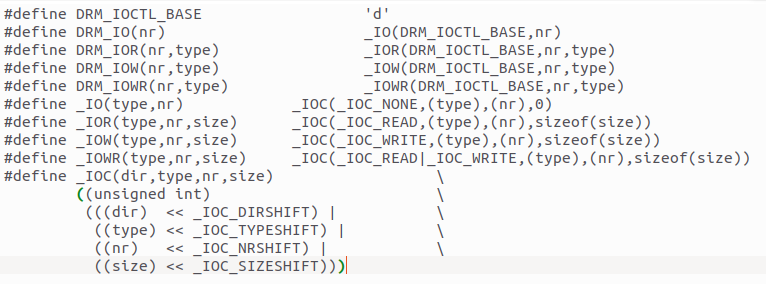
\includegraphics[width=0.8\textwidth]{IOCTL辅助宏定义.png}
%   \caption{IOCTL辅助宏定义}
%   \label{fig:IOCTL辅助宏定义}
% \end{figure}

在课题场景下,需要将内核调用的结果返回,因此使用双向的数据传输作为基础,实现GSGPU的ioctl。
为了给用户态程序提供创建和管理 GEM(图形内存对象)到处理上下文、命令流、内存映射、调度等支持,定义了如表\ref{tab:IOCTL命令码表}ioctl命令码。

\begin{table}[h]  
  \centering
  \caption{IOCTL命令码表}
  \label{tab:IOCTL命令码表}
  \resizebox{\linewidth}{!}{
  \begin{tabular}{llll}
    \toprule
    序号​	&​ 命令​ &​ 功能领域​	& 映射函数 \\
    \midrule
    0x00	& DRM\_GSGPU\_GEM\_CREATE	& ​GEM 内存管理​ & gsgpu\_gem\_create\_ioctl \\
    0x01	& DRM\_GSGPU\_GEM\_MMAP	& ​内存映射​ & gsgpu\_gem\_mmap\_ioctl \\
    0x02	& DRM\_GSGPU\_CTX	& ​上下文管理​	& gsgpu\_ctx\_ioctl\\
    0x03	& DRM\_GSGPU\_BO\_LIST	& ​缓冲区对象列表​	& gsgpu\_bo\_list\_ioctl\\
    0x04	& DRM\_GSGPU\_CS	& ​命令流控制​	& gsgpu\_cs\_ioctl\\
    0x05	& DRM\_GSGPU\_INFO	& ​设备信息查询​	& gsgpu\_info\_ioctl\\
    0x06	& DRM\_GSGPU\_GEM\_METADATA	& ​元数据管理​	& gsgpu\_gem\_metadata\_ioctl\\
    0x07	& DRM\_GSGPU\_GEM\_WAIT\_IDLE	& ​同步与闲置状态​	& gsgpu\_gem\_wait\_idle\_ioctl\\
    0x08	& DRM\_GSGPU\_GEM\_VA	& ​虚拟地址分配​	& gsgpu\_gem\_va\_ioctl\\
    0x09	& DRM\_GSGPU\_WAIT\_CS	& ​命令流同步​	& gsgpu\_cs\_wait\_ioctl\\
    0x10	& DRM\_GSGPU\_GEM\_OP	& ​通用 GEM 操作​	& gsgpu\_gem\_op\_ioctl\\
    0x11	& DRM\_GSGPU\_GEM\_USERPTR	& ​用户指针支持​	& gsgpu\_gem\_userptr\_ioctl\\
    0x12	& DRM\_GSGPU\_WAIT\_FENCES	& ​栅栏同步​	& gsgpu\_cs\_wait\_fences\_ioctl\\
    0x13	& DRM\_GSGPU\_VM	& ​虚拟内存管理​	& gsgpu\_vm\_ioctl\\
    0x14	& DRM\_GSGPU\_FENCE\_TO\_HANDLE	& ​栅栏与句柄映射​	& gsgpu\_cs\_fence\_to\_handle\_ioctl\\
    0x15	& DRM\_GSGPU\_SCHED	& ​任务调度​	& gsgpu\_sched\_ioctl\\
    0x16	& DRM\_GSGPU\_HWSEMA\_OP	& ​硬件信号量操作​	& gsgpu\_hw\_sema\_op\_ioctl\\
    \bottomrule
    \end{tabular}
  }
  \note{}
\end{table}

\begin{enumerate}[1)]
  \item GSGPU\_GEM\_CREATE:在内核中为GPU设备分配并初始化一个GEM对象。
  \item GSGPU\_GEM\_MMAP:将GEM对象映射到用户空间,允许用户态直接访问显存。
  \item GSGPU\_CTX:创建/销毁GPU上下文,管理上下文资源。
  \item GSGPU\_BO\_LIST:管理一组缓冲区对象操作的集合,用于批量操作。
  \item GSGPU\_CS:提交命令流到GPU硬件执行。
  \item GSGPU\_INFO:查询GPU硬件参数
  \item GSGPU\_GEM\_METADATA:设置/获取GEM对象的元数据,主要用于tiling模式或者缓存策略的选择。
  \item GSGPU\_GEM\_WAIT\_IDLE:等待GEM对象关联的所有GPU操作完成。
  \item GSGPU\_GEM\_VA:管理GEM对象的虚拟地址绑定,控制GPU虚拟地址空间映射。
  \item GSGPU\_WAIT\_CS:等待指定命令流完成执行。
  \item GSGPU\_GEM\_OP:对GEM对象执行通用操作,包括创建信息、设置内存放置域等。
  \item GSGPU\_GEM\_USERPTR:通过用户态指针注册内存作为GEM对象,支持零拷贝数据传输。
  \item GSGPU\_WAIT\_FENCES:等待多个栅栏信号完成。
  \item GSGPU\_VM:GPU 虚拟化管理的基础接口。
  \item GSGPU\_FENCE\_TO\_HANDLE:将栅栏转换为句柄,支持跨进程同步。
  \item GSGPU\_SCHED:配置调度策略,更改命令流执行顺序。
  \item GSGPU\_HWSEMA\_OP:操作硬件信号量,控制硬件级资源争用。
\end{enumerate}
由于这些功能大部分需要双向数据传输,所以大部分的命令码使用辅助宏DRM\_IOWR,可以用公式表示为:

\#define DRM\_IOCTL\_ioctl

 DRM\_IOWR(DRM\_COMMAND\_BASE+DRM\_ioctl,union structIoctl)

其中ioctl对应某个命令码,以DRM\_GSGPU\_GEM\_CREATE为例,ioctl=GSGPU\_GEM\_CREATE,structIoctl表示该命令码对应的数据大小,
DRM\_IOCTL\_ioctl实际上就是经过DRM\_COMMAND\_BASE基地址偏移的命令码。
每个命令码都对应具体的函数实现,通过DRM系统提供的DRM\_IOCTL\_DEF\_DRV宏完成联系。
这个宏的作用是将驱动私有的 IOCTL 命令注册到 DRM 的统一命令表中,并关联对应的处理函数和权限标志。如图\ref{lst:drm-ioctl-drv}。
这里实际上将DRM命令、处理该命令的内核函数指针、权限标志和命令的字符串名称分别存入cmd、func、flags和name域,在内核模块进行PCI设备注册时,
将命令表封装进drm\_device结构体的数据中,并在用户态程序进行ioctl系统调用时根据DRM命令码调用对应的内核函数func实现。
DRM命令码与内核处理函数func的映射关系已在表\ref{tab:IOCTL命令码表}中展示。

\begin{lstlisting}[caption={DRM驱动IOCTL定义宏}, label={lst:drm-ioctl-drv}, escapechar=@]
  #define DRM_IOCTL_DEF_DRV(ioctl, func, _flags) \
      {                                           \
          .cmd    = DRM_IOCTL_NR(ioctl),          \
          .func   = func,                         \
          .flags  = _flags,                       \
          .name   = #ioctl                        \
      }
  \end{lstlisting}
  
% \begin{figure}[h]
%   \centering
%   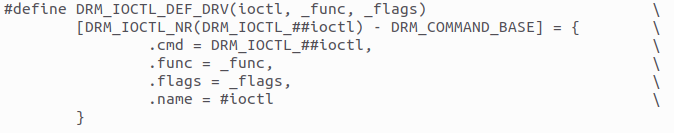
\includegraphics[width=0.8\textwidth]{ioctl def drv.png}
%   \caption{DRM\_IOCTL\_DEF\_DRV宏实现}
%   \label{fig:ioctl def drv}
% \end{figure}

% \subsection{内存管理模块}

% LG110的内存模型在小节\ref{sec:架构差异分析}和图\ref{fig:LG110内存模型}中已有相关说明。
% 模块主要功能是管理GPU显存资源(GEM对象)的创建、映射、元数据操作及虚拟地址绑定等。
% 其主要依赖GEM和TTM对缓冲区对象进行管理。
% GEM是内核中用于图形缓冲区管理的一个核心模块,特别是在与图形硬件(如 GPU)交互时。
% 它是 DRM的一部分,旨在为图形硬件分配、管理和共享内存资源。GEM 的设计目的是简化内存管理,确保图形缓冲区的高效分配和使用,并且能够支持多种类型的设备和硬件架构。
% GEM 主要通过图形缓冲区的对象(drm\_gem\_object)来管理 GPU 和显示硬件之间的内存。TTM(Translation Table Manager)适用于GPU内存管理的一部分,
% 提供了对显存、主存、共享内存等不同类型内存的管理功能。它通过一个通用的 API 提供内存分配、缓冲区对象管理和内存交换等功能,使得 GPU 驱动能够灵活管理图形资源。
% 在GPU内存管理中实际上不关心纹理会被分配到哪个内存,GPU内存会使用BO缓冲区对象去作为GPU显存使用的最小单位。
% 简单来说,GEM分配的显存对象底层drm\_gem\_object通过TTM的ttm\_buffer\_object管理物理内存。

% TTM实际上是使用GEM实现内存管理框架,在GEM模块实现了龙芯自己的数据结构,主要场景包括将VRAM转移到RAM或者从RAM转移到VRAM,以及BO的映射以实现CPU的访问。
% 还是得写ttm模块,突出5.10内核结构不同等等。
% \begin{figure}[h]
%   \centering
%   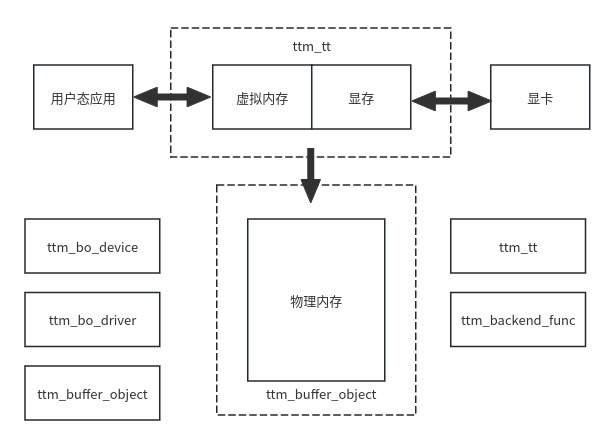
\includegraphics[width=0.8\textwidth]{DRM TTM结构.jpg}
%   \caption{TTM主要对象}
% \end{figure}

在DRM框架中,libdrm是沟通和连接内核空间和用户空间的重要一环。它通过对多种ioctl底层接口进行封装,以向上提供通用的接口。
用户空间的驱动可以通过libdrm提供的库函数与系统内核进行交互,从而访问底层资源。如图\ref{fig:内核驱动结构图},
libdrm\_gsgpu作为安卓用户空间的驱动程序,它会与底层的DRM内核驱动程序进行通信,
从而完成配置、读取、传输、控制设备等多种行为。

\begin{figure}[h]
  \centering
  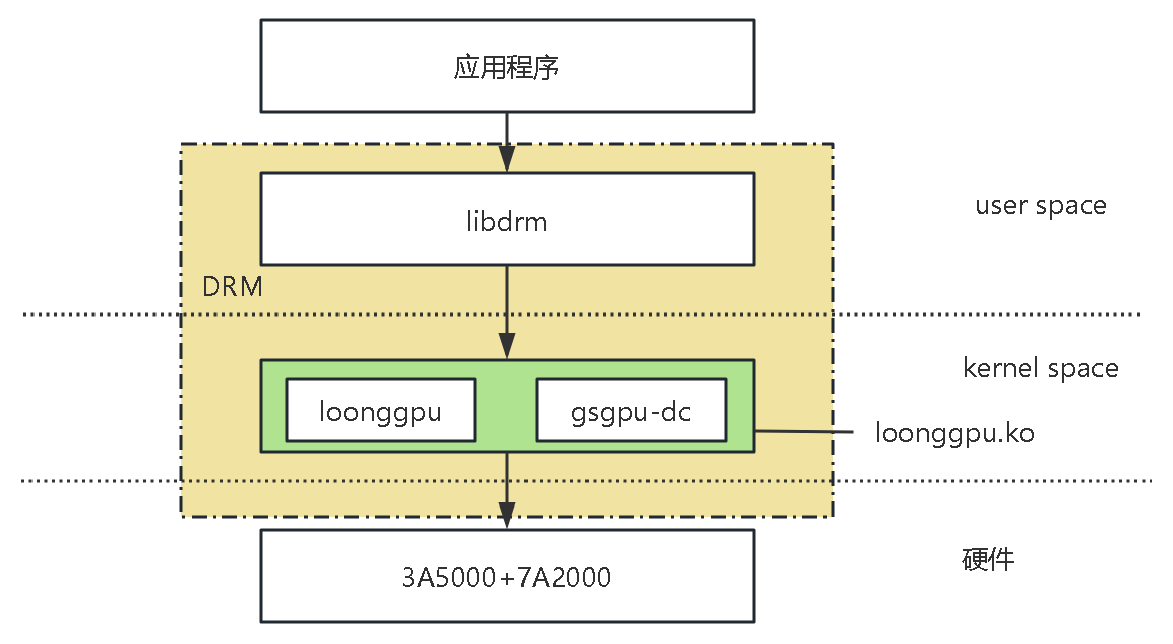
\includegraphics[width=0.8\textwidth]{内核驱动结构图.pdf}
  \caption{内核驱动结构图}
  \label{fig:内核驱动结构图}
\end{figure}

在libdrm中,用户态实现的缓冲区对象操作的函数
会通过drmCommandWriteRead封装的读写命令,对内核IOCTL实现进行调用。以gsgpu\_bo\_alloc为例,会在系统内存calloc一块BO缓冲区对象大小的内存,并通过
drmCommandWriteRead封装的args,以DRM\_IOC拆解传入的命令序号作为偏移值,以DRM\_COMMAND\_BASE作为基址获取命令编号,DRM\_IOCTL\_BASE作为操作类型,使用args的大小作为命令数据的大小,
方向默认双向,向内核请求特定的IOCTL操作,随后使用ioctl执行系统调用,操纵DRM设备。由此,实现了从用户态调用DRM命令码对显卡设备的操作。

% \begin{table}[h]
%   \centering
%   \caption{libdrmBO接口表}
%   \label{tab:libdrmBO接口表}
%   \begin{tabular}{ll}
%     \toprule
%     libdrm实现  & 命令序号 \\
%     \midrule
%     gsgpu\_bo\_alloc& DRM\_GSGPU\_GEM\_CREATE  \\
%     gsgpu\_bo\_cpu\_map & DRM\_GSGPU\_GEM\_MMAP \\
%     gsgpu\_bo\_cpu\_unmap & / \\
%     gsgpu\_bo\_export & / \\
%     gsgpu\_bo\_free & / \\
%     gsgpu\_bo\_import & / \\
%     gsgpu\_bo\_list\_create & DRM\_GSGPU\_BO\_LIST \\
%     gsgpu\_bo\_list\_destroy & DRM\_GSGPU\_BO\_LIST \\
%     gsgpu\_bo\_list\_update & DRM\_GSGPU\_BO\_LIST \\
%     gsgpu\_bo\_query\_info & DRM\_GSGPU\_GEM\_OP|DRM\_GSGPU\_GEM\_METADATA \\
%     gsgpu\_bo\_set\_metadata & DRM\_GSGPU\_GEM\_METADATA \\
%     gsgpu\_bo\_va\_op\_raw & DRM\_GSGPU\_GEM\_VA \\
%     gsgpu\_bo\_wait\_for\_idle & DRM\_GSGPU\_GEM\_WAIT\_IDLE \\
%     gsgpu\_create\_bo\_from\_user\_mem & DRM\_GSGPU\_GEM\_USERPTR \\
%     \bottomrule
%   \end{tabular}
%   \note{}
% \end{table}

\subsection{多版本适配方案设计}
龙芯gsgpu内核驱动属于闭源状态,尚未整合到已有的内核源码,采用的方案为驱动模块独立开发的方式,这样设计有多个方面的好处,

一是为了适应多种方式加载驱动模块的需求,既可以通过加载/lib/modules/\$(kernel\_uname)下
的内核源码头文件实现在已有的系统上动态编译驱动模块并通过DKMS(Dynamic Kernel Module Support)加载,实现在已运行的系统上完成显卡内核驱动模块的安装;也可以通过静态编译,
指定静态的源码树的位置并编译生成可加载的.ko驱动文件。由于安卓主要采用的是静态内核模块(built-in or prebuilt kernel modules)方式来管理驱动,
不支持原生的DKMS,因此本课题采用的是静态编译的方式,在源码树之外编译.ko驱动文件,并在进入安卓系统后使用insmod方式加载.ko驱动文件。

二是为了适应多种内核版本的需求,现龙芯平台主流内核版本为4.19、5.5或6.6,而本课题使用的安卓内核版本为5.10,内核驱动涉及的接口多有变化。
而gpu/drm模块的接口变化较多,这是因为显示模块由于硬件设计上的变化,内核模块的代码需要不断进行调整和优化,以适应现代GPU设备和复杂内存管理的需求。
如表\ref{tab:内核4.19-5.10 drm接口变化}所示,仅从4.19到5.10,drm模块的接口变化已有48项之多,这些接口上的变化导致具体的内核驱动模块需要不断更新迭代,耗时耗力。
因此在原有的4.19内核版本驱动的基础上进行多版本适配,即可以动态识别内核驱动版本接口,是非常有意义的。

\begin{table}[h]
  \centering
  \caption{内核4.19-5.10 drm接口变化}
  \label{tab:内核4.19-5.10 drm接口变化}
  \begin{tabular}{lll}
    \toprule
    类型   &   名称  &变化时内核版本  \\
    \midrule
    变量 & DRIVER\_PRIME & 5.4 \\
    变量 & DRIVER\_IRQ\_SHARED & 5.1 \\
    函数 & drm\_sched\_stop & 5.1 \\
    函数 & drm\_fb\_helper\_fill\_info & 5.2 \\
    变量 & glob(ttm\_bo\_device\_init) & 5.0 \\
    函数 & ttm\_resource\_manager & 5.9 \\
    ... & ... & ... \\
    \bottomrule
  \end{tabular}
  \note{共计48项}
\end{table}

由于drm模块的接口变化为某个函数的增加或删除,部分结构体的属性变化,以及函数的参数变化。以空参数调用某个函数时,若函数相关实现已被删除,则测试代码\textbf{不会产生}编译错误,
仅会在链接时产生错误,而函数存在时,则会产生编译错误,将此种情况命名为function;若某个函数的形参不存在或者结构体或者结构体的某个属性不存在时,则测试代码\textbf{会产生}编译错误,
此种情况命名为type。这两种情况存在和不存在时目标对象时编译结果完全相反,结果判断如表\ref{tab:测试代码判断表}所示。针对不同实现缺失的情形,返回的编译结果完全相反。

\begin{table}[h]
  \centering
  \caption{测试代码判断表}
  \label{tab:测试代码判断表}
  \begin{tabular}{lll}
    \toprule
    类型   &   编译结果 & 函数\&属性\&参数是否存在    \\
    \midrule
    function & 不通过 & 存在 \\
    function & 通过 & 不存在 \\
    type & 通过 & 存在 \\
    type & 不通过 & 不存在 \\
    \bottomrule
  \end{tabular}
\end{table}

具体的方式为实现一个conftest.sh的脚本,假使该目标宏定义为DEF,如算法\ref{algo:algorithm1}所示,通过尝试编译测试代码,测试代码中引入已有的内核头文件,并按以下数种情况实现测试代码:

1.某函数实现删除或增加,假设目标测试函数为funcB,使用一个空返回值空形参的测试函数funcTest并调用无参数的目标函数,可视funcA的返回值情况选择是否设置funcB的返回值,
如算法\ref{algo:algorithm2}所示。

2.某函数实现的形参删除或增加,沿用1假设,添加调用funcB所需的参数,调用funcB并返回,如算法\ref{algo:algorithm3}所示。

3.某结构体的删除或增加,假设目标结构体类型为A,在funcTest中使用A的形参即可,如算法\ref{algo:algorithm4}所示。

4.某结构体中属性的删除或增加,沿用3假设,目标结构体的目标属性为c,使用offsetof(offsetof是一个 C语言的宏,
主要用于计算 结构体成员相对于结构体起始地址的偏移量)测试该结构体是否存在属性c,如算法\ref{algo:algorithm5}所示。

通过编译测试代码的结果(即是否生成中间代码.o文件)以及相应的类型(即function或者type)判断是否存在相关实现,并以此为基础生成相应的宏头文件,为GPU内核驱动的具体实现中提供判断基础。

\begin{algorithm}[h]
  \SetAlgoLined
  ...\;
  将测试代码重定向至conftest.c\;
  尝试编译conftest.c并忽略异常输出\;
  \eIf{存在conftest.o文件}{
    \eIf{类型为function}{
      显示未定义DEF并将其重定向至头文件\;
    }{
      显示已定义DEF并将其重定向至头文件\;
    }
  }{
    \eIf{类型为type}{
      显示已定义DEF并将其重定向至头文件\;
    }{
      显示未定义DEF并将其重定向至头文件\;
    }
  }
  \caption{编译检查测试函数}
  \label{algo:algorithm1}
\end{algorithm}

\begin{minipage}{0.45\textwidth}
  \begin{algorithm}[H]
    \SetAlgoLined
    \KwData{void}
    \KwResult{TypefuncB}
    TypefuncB funcTest(void){\\
      return funcB()\;
        or \;
      funcB()\;
    }
    \caption{测试代码示例1}
    \label{algo:algorithm2}
  \end{algorithm}
\end{minipage}
\hfill
\begin{minipage}{0.45\textwidth}
  \begin{algorithm}[H]
    \SetAlgoLined
    \KwData{arg1,arg2,...}
    \KwResult{TypefuncB}
    TypefuncB funcTest(Type1 arg1,Type2 arg2,...){\\
      return funcB(arg1,arg2,...)\;
    }
    \caption{测试代码示例2}
    \label{algo:algorithm3}
  \end{algorithm}
\end{minipage}

\begin{minipage}{0.45\textwidth}
  \begin{algorithm}[H]
    \SetAlgoLined
    \KwData{TypeA}
    \KwResult{void}
    void funcTest(TypeA a){\\
      return \;
    }
    \caption{测试代码示例3}
    \label{algo:algorithm4}
  \end{algorithm}
\end{minipage}
\hfill
\begin{minipage}{0.45\textwidth}
  \begin{algorithm}[H]
    \SetAlgoLined
    \KwData{void}
    \KwResult{int}
    int funcTest(void){\\
      return offsetof(struct B,c) \;
    }
    \caption{测试代码示例4}
    \label{algo:algorithm5}
  \end{algorithm}
\end{minipage}


% \section{GPU用户态驱动实现}

% 龙芯现有的驱动实现基于mesa的gallium架构。
% gallium结构可以分为state tracker层,驱动层以及面向操作系统的Winsys层。
% state tracker是状态跟踪器,负责将将高级图形API的调用转换为Gallium内部的具体的管道操作。
% 而驱动层是直接与GPU硬件交互的部分,负责硬件指令生成,就是将Gallium的中间命令转换为GPU特定的指令集;着色器编译,将NIR中间表示编译为GPU原生代码,并进行优化;
% 资源管理,分配显存、管理纹理和缓冲区对象;命令提交,构建命令缓冲区,并通过winsys提交到硬件队列等。这是硬件特性的最直接体现,它和state tracker组成了
% gallium架构下实现OpenGL ES功能的核心组件。
% 而winsys层主要包括显存管理、命令提交与同步、显示输出管理和操作系统平台适配上。因此本课题主要实现在于winsys层模块的部分重构,而OpenGL ES实现复用
% 驱动层的实现即可。

\section{硬件混合渲染模块}
%每个厂商hwc实现可能不同如nxp,rockchip,drm-hwc,ranchu,也有很多厂商实现是闭源的如nxp,而谷歌的drm-hwc,ranchu是开源的

\begin{figure}[H]
  \centering
  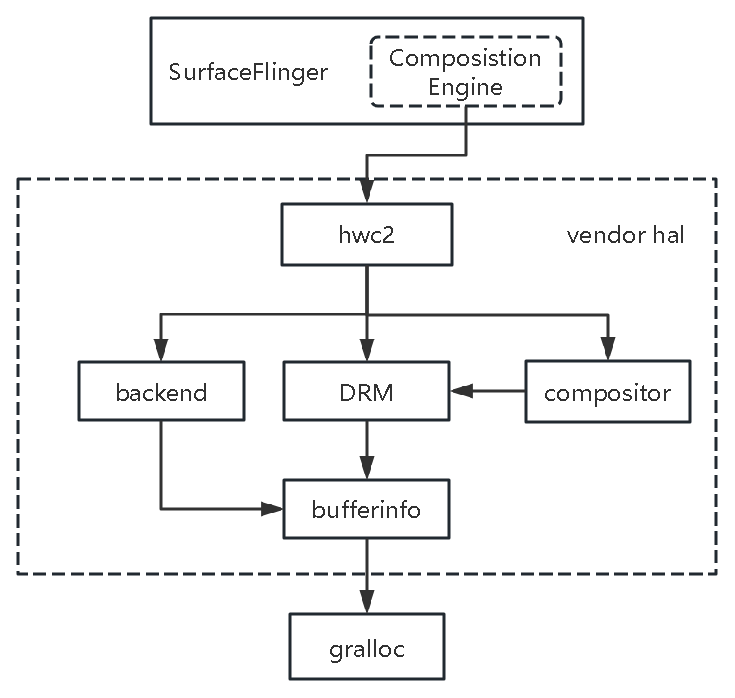
\includegraphics[width=0.6\textwidth]{HWC模块结构.pdf}
  \caption{HWC模块结构}
  \label{fig:HWC模块结构}
\end{figure}

\subsection{主要模块}

\subsubsection{DRM管理模块}
该模块是硬件混合渲染器的核心模块,负责直接与 Linux DRM/KMS(Direct Rendering Manager/Kernel Mode Setting)子系统交互,管理显示硬件资源,
定义了一系列与DRM相关的资源类,如DRM设备抽象、原子提交状态管理、硬件资源对象(Connector/CRTC/Plane/Encoder)、帧缓冲导入等。封装了
原子提交(Atomic Commit)、帧缓冲管理(DrmFbImporter)、资源管理(ResourceManager)、VSync 事件处理(VSyncWorker)、显示管线配置(DrmDisplayPipeline)等一系列功能。

该模块依赖缓冲区信息模块解析图形缓冲区的硬件属性。

\subsubsection{HWC2接口模块}
该模块通过实现HWC2标准定义的接口(如hwc2\_device\_t结构体中的函数指针),将SurfaceFlinger传递的图层数据转化为针对特定显示硬件的合成操作。
其主要工作流程始于Android图形系统的合成请求,通过prepare阶段评估各图层的合成可行性,利用硬件覆盖平面(Overlay Plane)优化性能,避免不必要的GPU参与,
最终在present阶段通过DRM原子提交将配置好的显示帧推送至屏幕。

模块内部通过HwcDisplay类管理单个物理显示设备的状态,包括分辨率、刷新率等显示属性的动态配置,同时处理热插拔事件与多显示器协同工作。
每个图层由HwcLayer对象封装,负责解析Android传递的缓冲区句柄、混合模式及变换矩阵,并通过BufferInfoGetter与底层Gralloc实现交互,获取像素格式、
步长(stride)及DMA-BUF文件描述符等关键元数据。当硬件资源分配时,该模块与合成策略模块(如DrmKmsPlan)协同,决策如何将图层分配到不同的DRM平面
(如Primary Plane用于主图层,Overlay Plane用于视频叠加),并处理缩放、旋转等硬件加速特性。

该模块依赖于后端管理模块、合成器模块以及DRM管理模块

\subsubsection{合成器模块}
该模块主要完成DrmKmsPlan的创建,在创建计划时通过对显示管线中的所有plane(平面)格式判断是否符合上层创建的Layer(图层)的需求,若符合则将设置plane、Layer、zpos(图层的顺序)
等参数并将新的计划加入显示队列。

该模块依赖于DRM管理模块。

\subsubsection{缓冲区信息适配模块}
该模块主要用于获取不同硬件厂商的Gralloc实现,并提供统一接口获取图形缓冲区的元数据。主要使用hw\_get\_module,以GRALLOC\_HARDWARE\_MODULE\_ID(Android中gralloc模块的标识符
)来加载Gralloc模块。

该模块由于是从Android硬件抽象层加载模块,所以不依赖于任何模块

\subsubsection{后端管理模块}
前段接口功能的内部实现,包括验证显示设备的状态、获取客户端图层的范围、检查硬件是否支持特定类型的合成、计算图形操作数计算、需要额外由客户端处理的层范围等,其中较为主要的是实现了
验证显示设备的状态(ValidateDisplay)方法,属于显示验证阶段的核心逻辑,用于决定哪些图层(Layer)可以被硬件直接合成(Overlay),哪些需要回退到 GPU 合成(Client Composition)。

该模块依赖于缓冲区信息适配模块。

\subsection{实现细节}

\subsubsection{设备注册与初始化}

这一部分的内容主要是DRM管理模块完成,在创建hwcomposer回调时,首先完成对DRM设备资源的初始化,,需要先打开/dev/dri/card*设备文件,
使用drmSetClientCap方法设置DRM客户端能力标志,用于支持通过统一的接口访问和管理所有类型的显示平面,
并启用和指示图形硬件支持原子操作,使用drmGetCap方法检查是否支持framebuffer 修饰符功能。随后获取DRM设备的主控制权,使用drmModeGetResources方法获取DRM设备的资源,
如CRTCs(显示控制器),encoders(编码器),connectors(连接器)并初始化,显示控制器和编码器初始化较为简单,其实就是分别调用drmModeCrtc、drmModeEncoder并储存返回的
指针。而连接器则需要在使用drmModeConnector获取链接器资源后,检查连接器的DPMS(显示电源管理信号)和CRTC\_ID(显示控制器id)是否正常,EDID(扩展显示识别数据)获取显示设备的能力。
在此之后,需要判断连接器是否支持写回(writeback),以及是否支持写回像素格式、framebuffer 的 ID以及输出同步的栅栏指针等这些属性这些都成功后才能储存连接器的指针。
随后使用drmModePlaneRes获取所有的平面(plane),在初始化时获取平面类型(OVERLAY、PRIMARY、CURSOR),并获取一些与显示控制器、帧缓冲、坐标、大小等相关的设置。事实上,由于龙芯
目前的硬件仅支持PRIMARY和CURSOR平面类型,较为简易,在此不再赘述。若上述过程都无异常则初始化成功完成。

\subsubsection{帧缓冲区合成}
该部分主要是将输入缓冲区对象转换为GEM句柄,从降低系统开销的目标出发设计了转换缓存表,首先需要调用 drmPrimeFDToHandle 接口将文件描述符映射为当前DRM设备可识别的显存资源标识符。
对缓存表中已存在的句柄进行查找,若缓存命中则直接返回,若缓存未命中则创建一个新的帧缓冲对象。首先解析缓冲区是否为多平面结构,
将每个非零且不与首个平面重复的 DMA-BUF通过drmPrimeFDToHandle转换为独立的GEM句柄,并通过drmModeAddFB2接口注册帧缓冲区。
在创建帧缓冲区实例后,以GEM句柄为键值,存入缓存,以供后续使用。

\subsubsection{原子提交}
原子提交主要是用于当前帧向DRM系统提交进行画面更新。其主要流程包括显示状态预与初始化、原子属性集构建、图层平面分配与状态注入、原子提交执行、提交后状态同步5个阶段。
显示状态预检与初始化主要是对当前显示控制器状态进行激活并创建新的帧状态对象,并关联至DRM设备、连接器与显示控制器,为后续属性配置提供上下文。原子属性集构建通过
drmModeAtomicFree属性状态清空、drmModeAtomicAddProperty设置同步栅栏以及显示控制器ID等一系列属性。图层平面分配与状态注入包括遍历每个图层,依次执行平面的原子状态设置
并将图层的帧缓冲区句柄关联至平面。原子提交执行是调用 drmModeAtomicCommit提交属性集。提交后同步是更新新的帧状态,传递输出栅栏至调用方,供渲染引擎或合成器同步后续操作。

\subsubsection{验证与显示}
实际上,hwcomposer的客户端调用是在SurfaceFlinger中,通过显示钩子函数实现对服务端具体功能的调用。
由于龙芯目前的硬件不支持硬件混合渲染,所以SurfaceFlinger的画面合成过程实际上是基于OpenGL ES完成的,是使用client模式合成,仅使用了HWComposer1.0接口标准的软件实现
也就是使用renderengine(课题使用的是支持了龙芯驱动的skia渲染引擎)合成。
这里的client合成是相对于HWC硬件合成而言的,其合成方式是将layer的内容用GPU渲染到缓冲区,然后由缓冲区送显到显示控制器。
其基本过程是首先获取显示设备支持的所有layer,并判断是否支持上层的需求,随后使用CreateComposition尝试创建合成(事实上在后续present送显时也是调用这个函数),若创建成功则更新
像素操作数等统计信息并返回结果。
在CreateComposition时,会初始化渲染管道pipe,按照zpos排列图层并导入帧缓冲区,为图层创建DrmKms计划,并进行画面更新。


% 1.HWC合成周期
% \begin{figure}[h]
%   \centering
%   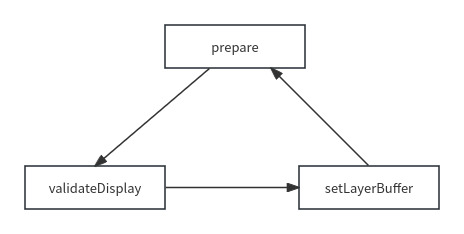
\includegraphics[width=0.8\textwidth]{HWC周期.jpg}
%   \caption{HWC周期}
%   \label{fig:HWC周期}
% \end{figure}

% 准备阶段:
% 每当屏幕内容需要更新时,SurfaceFlinger 会调用 prepare 函数,遍历所有图层并标记它们的合成方式(通过硬件加速device方式还是通过 GPU 合成client方式)。
% 此时会根据图层内容的变化(例如 UI 更新、视频播放等)重新评估每个图层的合成方式
% 验证与提交阶段:
% 在每次显示刷新之前,SurfaceFlinger 会调用 validateDisplay 来检查当前的显示配置是否可以创建DrmKms计划,以检查硬件是否支持。
% 如果硬件支持,则生成 DrmKmsPlan 并准备提交显示计划(调用 presentDisplay提交DRM原子操作)。如果硬件不支持,则回退到 GPU 合成
% 图层提交阶段:
% 在提交图层时,SurfaceFlinger 会使用 setLayerBuffer 更新每个图层的缓冲区,并通过 DrmFbImporter 将 Gralloc Buffer 转换为 DRM Framebuffer。
% 这些 Framebuffer 会被绑定到相应的 DRM Plane,然后将图层显示到屏幕上。

% 2.设备监测
% 显示器热插拔:

% UEventListener 检测到 HDMI 插入 → ResourceManager 重新扫描 Connector → 通知 HWC2 模块更新显示配置。

% 提交显示配置:

% HWC2 调用 DrmAtomicStateManager → 配置 Connector 的 CRTC、Plane 属性 → 提交原子操作。

% 帧缓冲处理:

% DrmFbImporter 将 Android Buffer 转换为 drm\_fb → 绑定到 Plane 的 FB\_ID 属性。


\section{图形缓存分配模块}
由于Android系统主要用于arm架构,而arm架构下的GPU多数没有自己的独立显存,系统服务SurfaceFlinger申请的帧缓存属于系统内存,而在本课题中,LoongArch架构下,
GSGPU有自己的专属独立显存。因此首先要解决的是如何让Android的SurfaceFlinger能够在LoongArch架构下运行,而SurfaceFlinger依赖的缓冲区管理的HAL实现就是gralloc。
依照Android 12的gralloc标准,gralloc模块接口定义有两部分,分别是mapper和allocator,
位于AOSP源码结构下的hardware/interface/graphic/mapper以及hardware/interface/graphic/allocator,
其中定义了缓冲区的描述符的数据结构,创建、导入、释放缓冲区对象等。本节按照hal文件定义的接口实现了一个绑定式图形缓存分配器。

gralloc模块的HAL服务有绑定式(Binderized )也有直通式(Passthrough),区别在于,直通式会被编译成.so库文件,为system和vendor分区的进程和应用在运行时动态加载调用,两者是在
同一进程中,而绑定式会被编译成一个可独立运行的服务,类似于一个守护进程,然后相关服务进程或应用会通过HwBinder的IPC(进程间通信)方式来调用,是在两个独立的进程中。绑定式是Google
在Android8.0时,为了方便升级系统框架所做的解耦技术。而绑定式又有默认直通式实现(defaultPassthroughServiceImplementation)以及 注册成服务(RegisterAsService)
两种类型,本课题采用的是第二种。在具体的实现上,采用VINTF Fragments为本模块创建清单并与相应的hal相关联,并且需要设置rc文件并安装到/vendor/etc/init目录下,为init进程初始化
提供执行依据(init进程会在加载init.rc主目录后立即加载/system/etc/init、/vendor/etc/init、/odm/etc/init等相关目录中的文件)。

\begin{figure}[h]
  \centering
  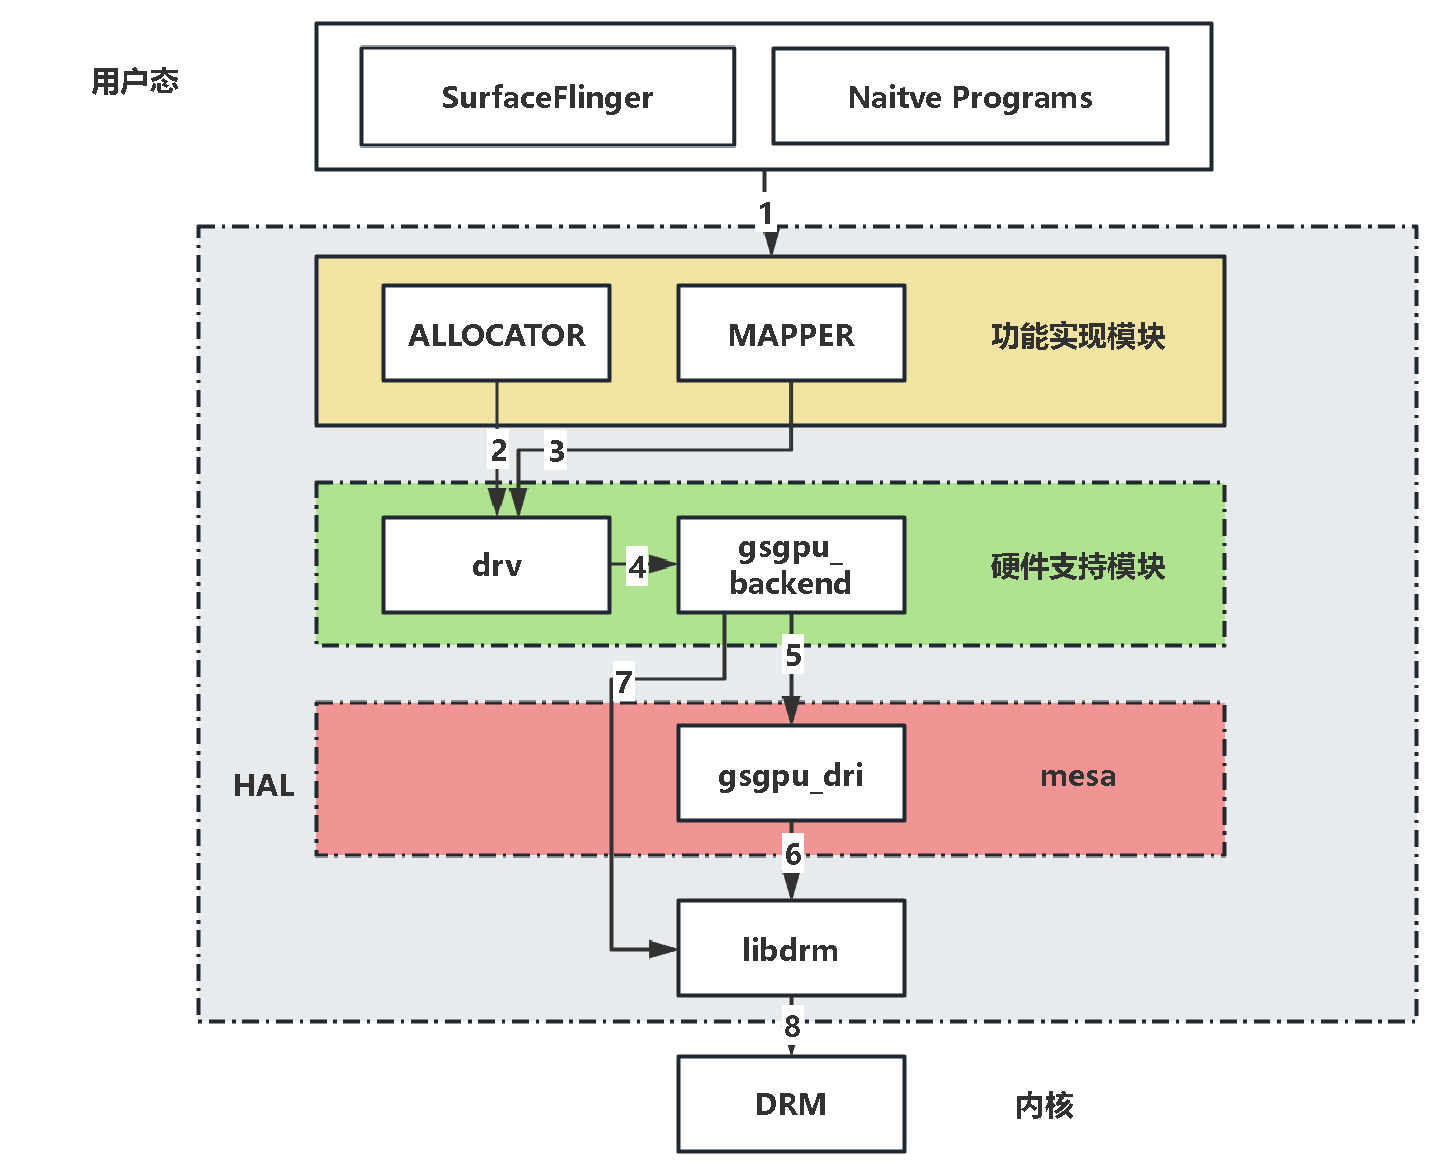
\includegraphics[width=0.8\textwidth]{gralloc调用栈v2.pdf}
  \caption{gralloc调用栈}
  \label{fig:gralloc调用栈}
\end{figure}

Android自身提供了共享内存的机制,native\_handle\_t是一个用于描述缓冲区的结构体,可以在进程之间传递缓冲区信息,gralloc\_handle\_t是Android 图形缓冲区分配器(Gralloc)中的句柄结构,
它继承自 native\_handle\_t,用于管理共享图形缓冲区。gralloc\_handle\_t这一特性需要libdrm的支持,最低版本需要2.4.97之后才支持此特性,目前龙芯已有的libdrm的解决方案已有2.4.97,
满足相关支持。
然后gralloc\_handle\_t图形缓冲区的创建如图\ref{fig:gralloc调用栈}所示,分为gralloc前端和后端,使用一个drv作为中间层(主要是gralloc实现的一些辅助函数),具体实现会调用支持了
gsgpu的后端库,该后端包含的缓冲区操作函数如\ref{tab:gralloc模块后端接口表}。Android系统上层应用程序在需要使用图形缓存时,使用路径1通过IPC跨进程通信向gralloc守护进程申请图形缓存,
然后allocator和mapper会通过路径(2-3)调用drv辅助函数,辅助函数相关实现通过路径4基于gsgpu\_backend实现,该后端会通过路径5基于gsgpu的DRI驱动或者直接通过路径6调用libdrm的IOCTL命令,
gsgpu DRI驱动会通过路径6调用集成在libdrm的接口函数,libdrm通过路径8实现用户态程序和DRM内核的交互。

\begin{table}[h]  
  \centering
  \caption{gralloc模块后端接口表}
  \label{tab:gralloc模块后端接口表}
  \begin{tabular}{ll}
    \toprule
    接口名  & 作用\\
    \midrule
    init\&close & 驱动程序的初始化和关闭 \\
    bo create & 创建缓冲区对象(BO)的函数,实现内存分配和初始化 \\
    bo destroy & 销毁缓冲区对象的函数,负责释放已分配的内存 \\
    bo import & 导入缓冲区对象的函数,允许将外部缓冲区导入到 GBM 管理的缓冲区中 \\
    bo map & 映射缓冲区对象的函数,使得 CPU 可以访问 GPU 分配的内存 \\
    bo unmap & 解除映射缓冲区对象的函数,释放 CPU 对缓冲区的访问 \\
    ... & ... \\
    \bottomrule
  \end{tabular}
  \note{}
\end{table}

\subsection{硬件支持模块}

为了实现高效调度,龙芯后端实现部分基于libdrm模块drmCommandWrite等直接与DRM内核进行通信,其具体原理已在\ref{sec:IOCTL命令码设计}中所述。

\subsubsection{驱动初始化与关闭模块}

在对驱动硬件进行调用前,首先需要初始化GSGPU硬件信息,使用query\_dev\_info(实际上使用DRM接口查询GSGPU\_INFO);随后加载gsgpu的DRI驱动,
通过drmGetRenderDeviceNameFromFd解析DRM渲染节点路径,通过dlopen加载gsgpu\_dri.so动态库,解析符号表获取扩展接口,
调用createNewScreen2初始化Mesa内部状态机,关联DRM设备节点,注册硬件特性,并通过createNewContext创建线程安全的渲染上下文,支持多API共享;
同时激活\_\_DRI\_IMAGE相关拓展功能。若某一阶段失败,则依次销毁已创建的上下文、屏幕对象,关闭设备节点并卸载驱动库,防止资源泄漏。
并且初始化XDMA引擎,首先是硬件兼容性检查,通过GSGPU\_CTX命令创建硬件上下文,隔离SDMA操作的执行环境,以支持多任务并行提交;同时创建
命令缓冲区,使用GSGPU\_GEM\_CREATE创建GEM对象,并指定域为GSGPU\_GEM\_DOMAIN\_GTT,即系统内存;随后使用GSGPU\_GEM\_VA将命令缓冲区映射到GPU虚拟地址空间,
并设置权限为可读/可执行;通过GSGPU\_GEM\_MMAP获取缓冲区的物理地址,使用mmap将其映射到用户态,支持驱动直接写入XDMA命令。
而在缓冲区格式配置中,主要是配置一些渲染格式、纹理格式、光标格式与缓冲区标志相对应,常见的缓冲区类型如\ref{tab:缓冲区标志表},
这些标志用于标识缓冲区的不同使用场景,通常在图形和视频处理系统中使用。每个标志代表缓冲区的不同用途,允许驱动程序和硬件根据不同的用途进行优化或操作。

\begin{table}[h]  
  \centering
  \caption{缓冲区标志表}
  \label{tab:缓冲区标志表}
  \begin{tabular}{ll}
    \toprule
    接口名  & 作用\\
    \midrule
    BO\_USE\_NONE & 表示没有任何用途。通常用于初始化或不需要使用标志的情况 \\
    BO\_USE\_SCANOUT & 该标志表示缓冲区将用于显示输出 \\
    BO\_USE\_CURSOR & 该标志表示缓冲区将用于显示光标 \\
    BO\_USE\_RENDERING & 该标志表示缓冲区将用于渲染操作 \\
    BO\_USE\_LINEAR & 该标志表示缓冲区的内存布局是线性的 \\
    BO\_USE\_TEXTURE & 该标志表示缓冲区将作为纹理使用 \\
    ... & ... \\
    \bottomrule
  \end{tabular}
  \note{}
\end{table}

在驱动关闭时,需要对使用的资源进行释放,XDMA引擎关闭时需要解除命令缓冲区映射,使用GSGPU\_GEM\_VA命令的VA\_OP\_UNMAP操作解除GPU虚拟地址映射​,
同时使用GSGPU\_GEM\_CLOSE关闭命令缓冲区的GEM对象句柄,并释放SDMA硬件上下文​。随后是DRI驱动资源释放,需要销毁渲染上下文和屏幕对象,并卸载DRI驱动库,并
关闭设备节点。整体结构如图\ref{fig:lgbm后端-1}所示。

\begin{figure}[h]
  \centering
  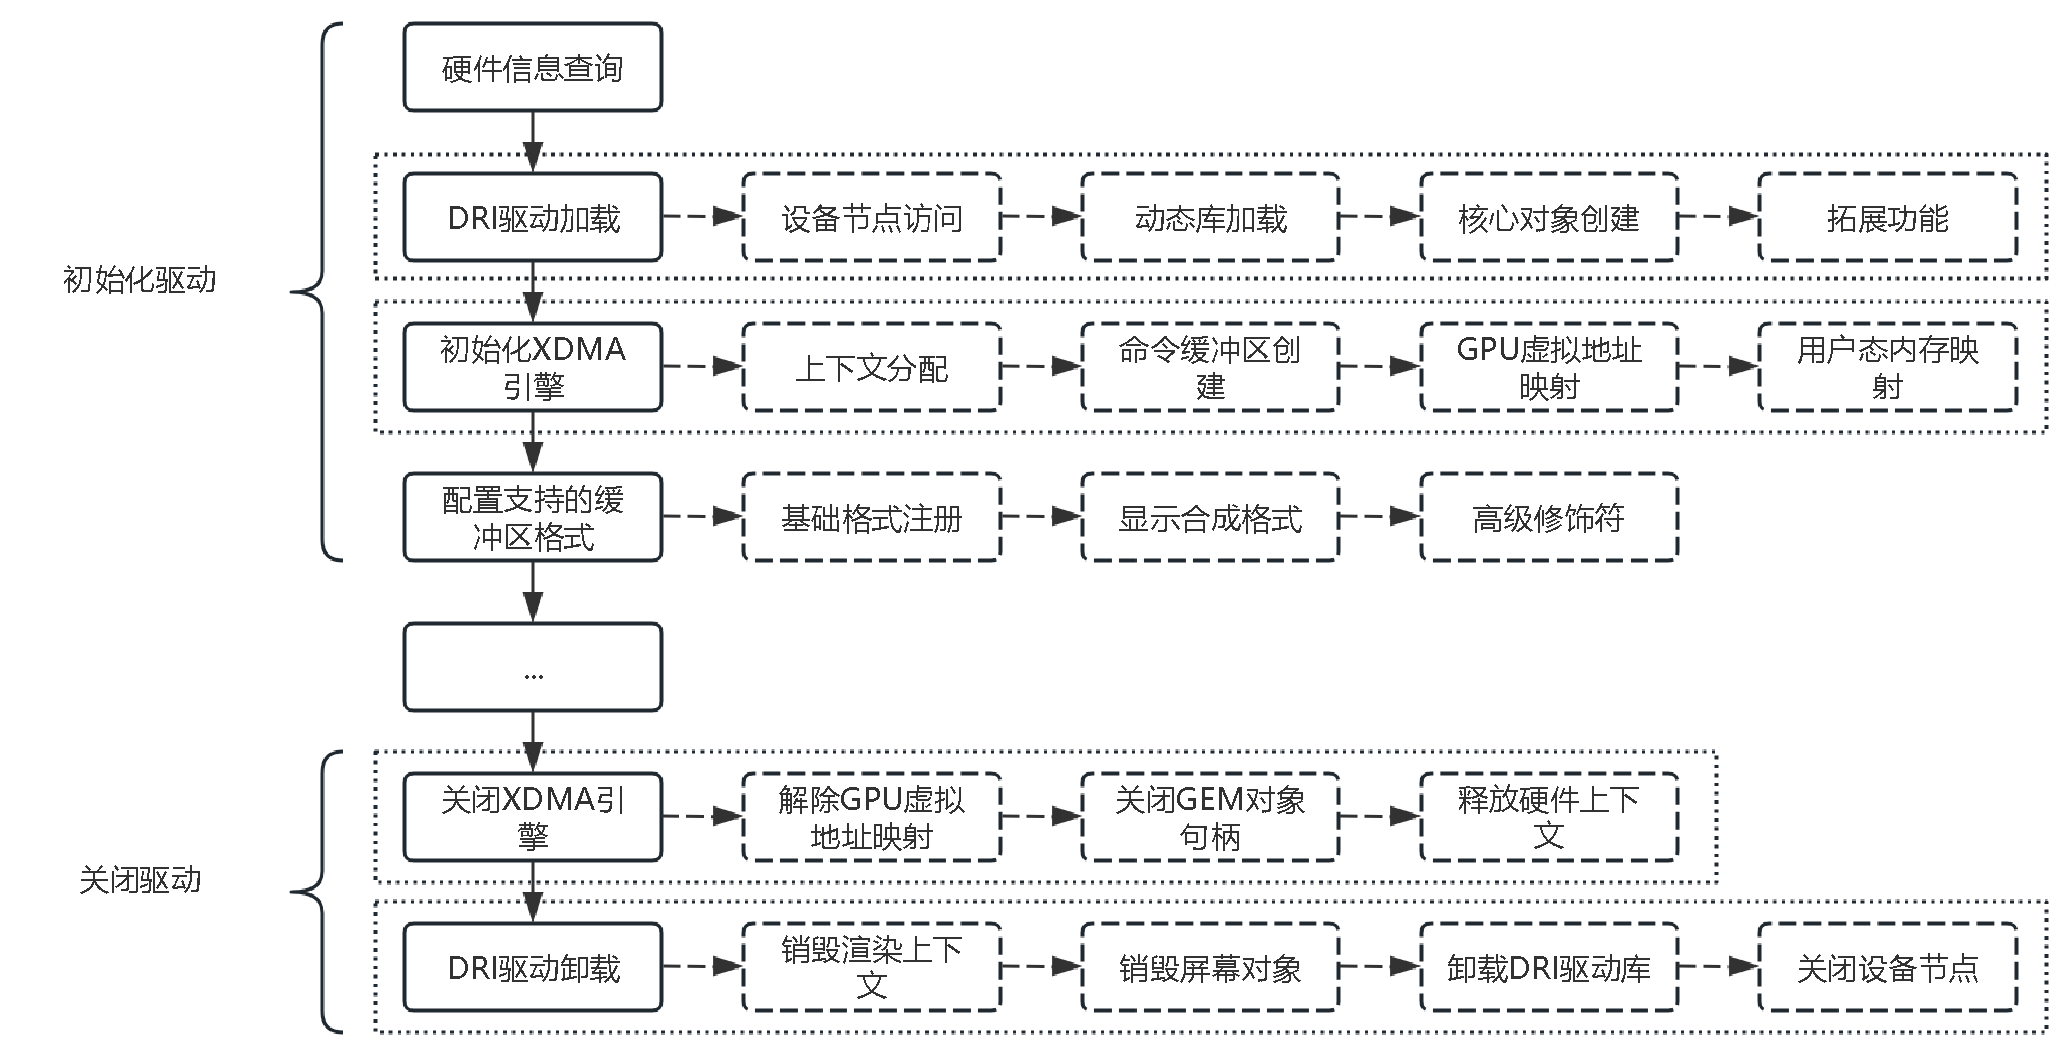
\includegraphics[width=1\textwidth]{lgbm后端-1.pdf}
  \caption{驱动初始化与关闭}
  \label{fig:lgbm后端-1}
\end{figure}  

\subsubsection{内存传输加速模块}

独立处理GPU加速的内存传输操作,利用了LG110硬件XDMA的特性,实现从一个源内存地址到目标内存地址的数据搬运,支持Linear和Tiled 数据格式存储。
首先需要校验参数与准备资源,计算能处理的最大命令数量(不能超过最大单次传输尺寸)。其次将源缓冲区和目标缓冲区分别通过GSGPU\_GEM\_VA的VA\_OP\_MAP映射到GPU的虚拟空间,以便于从GPU中获取这两个地址,
但是在目标缓冲区上添加WRITEABLE标志表示这是写入的标志。随后构造XDMA命令如\ref{tab:XDMA描述符},按顺序构造完命令后循环构造DMA命令。
在构造完DMA命令后,设置指令缓冲区指定命令缓冲区的起始地址以及设置硬件类型为XDMA,随后构造提交这批次DMA命令的命令块,主要是封装之前构建的DMA命令和
指令缓冲区,随后通过GSGPU\_CS将命令块提交到硬件,并等待结果同步,进行超时或调用错误等处理。流程如图\ref{fig:lgbm后端-2}所示。

\begin{table}[h]  
  \centering
  \caption{XDMA描述符}
  \label{tab:XDMA描述符}
  \begin{tabular}{lll}
    \toprule
    名称  & 偏移 & 描述\\
    \midrule
    CONTROL & 0x00 & 操作控制\\
    SIZE & 0x04 & 传输尺寸\\
    DST\_ADDR\_LO & 0x08 & 目标缓冲区低位\\
    DST\_ADDR\_HI & 0x0c & 目标缓冲区高位\\
    SRC\_ADDR\_LO & 0x10 & 源目标缓冲区低位\\
    SRC\_ADDR\_HI & 0x14 & 源目标缓冲区高位\\
    DST\_STRIDE & 0x18 & 目标缓冲区行跨度\\
    SRC\_STRIDE & 0x1c & 源缓冲区行跨度\\
    \bottomrule
  \end{tabular}
  \note{}
\end{table}

\begin{figure}[h]
  \centering
  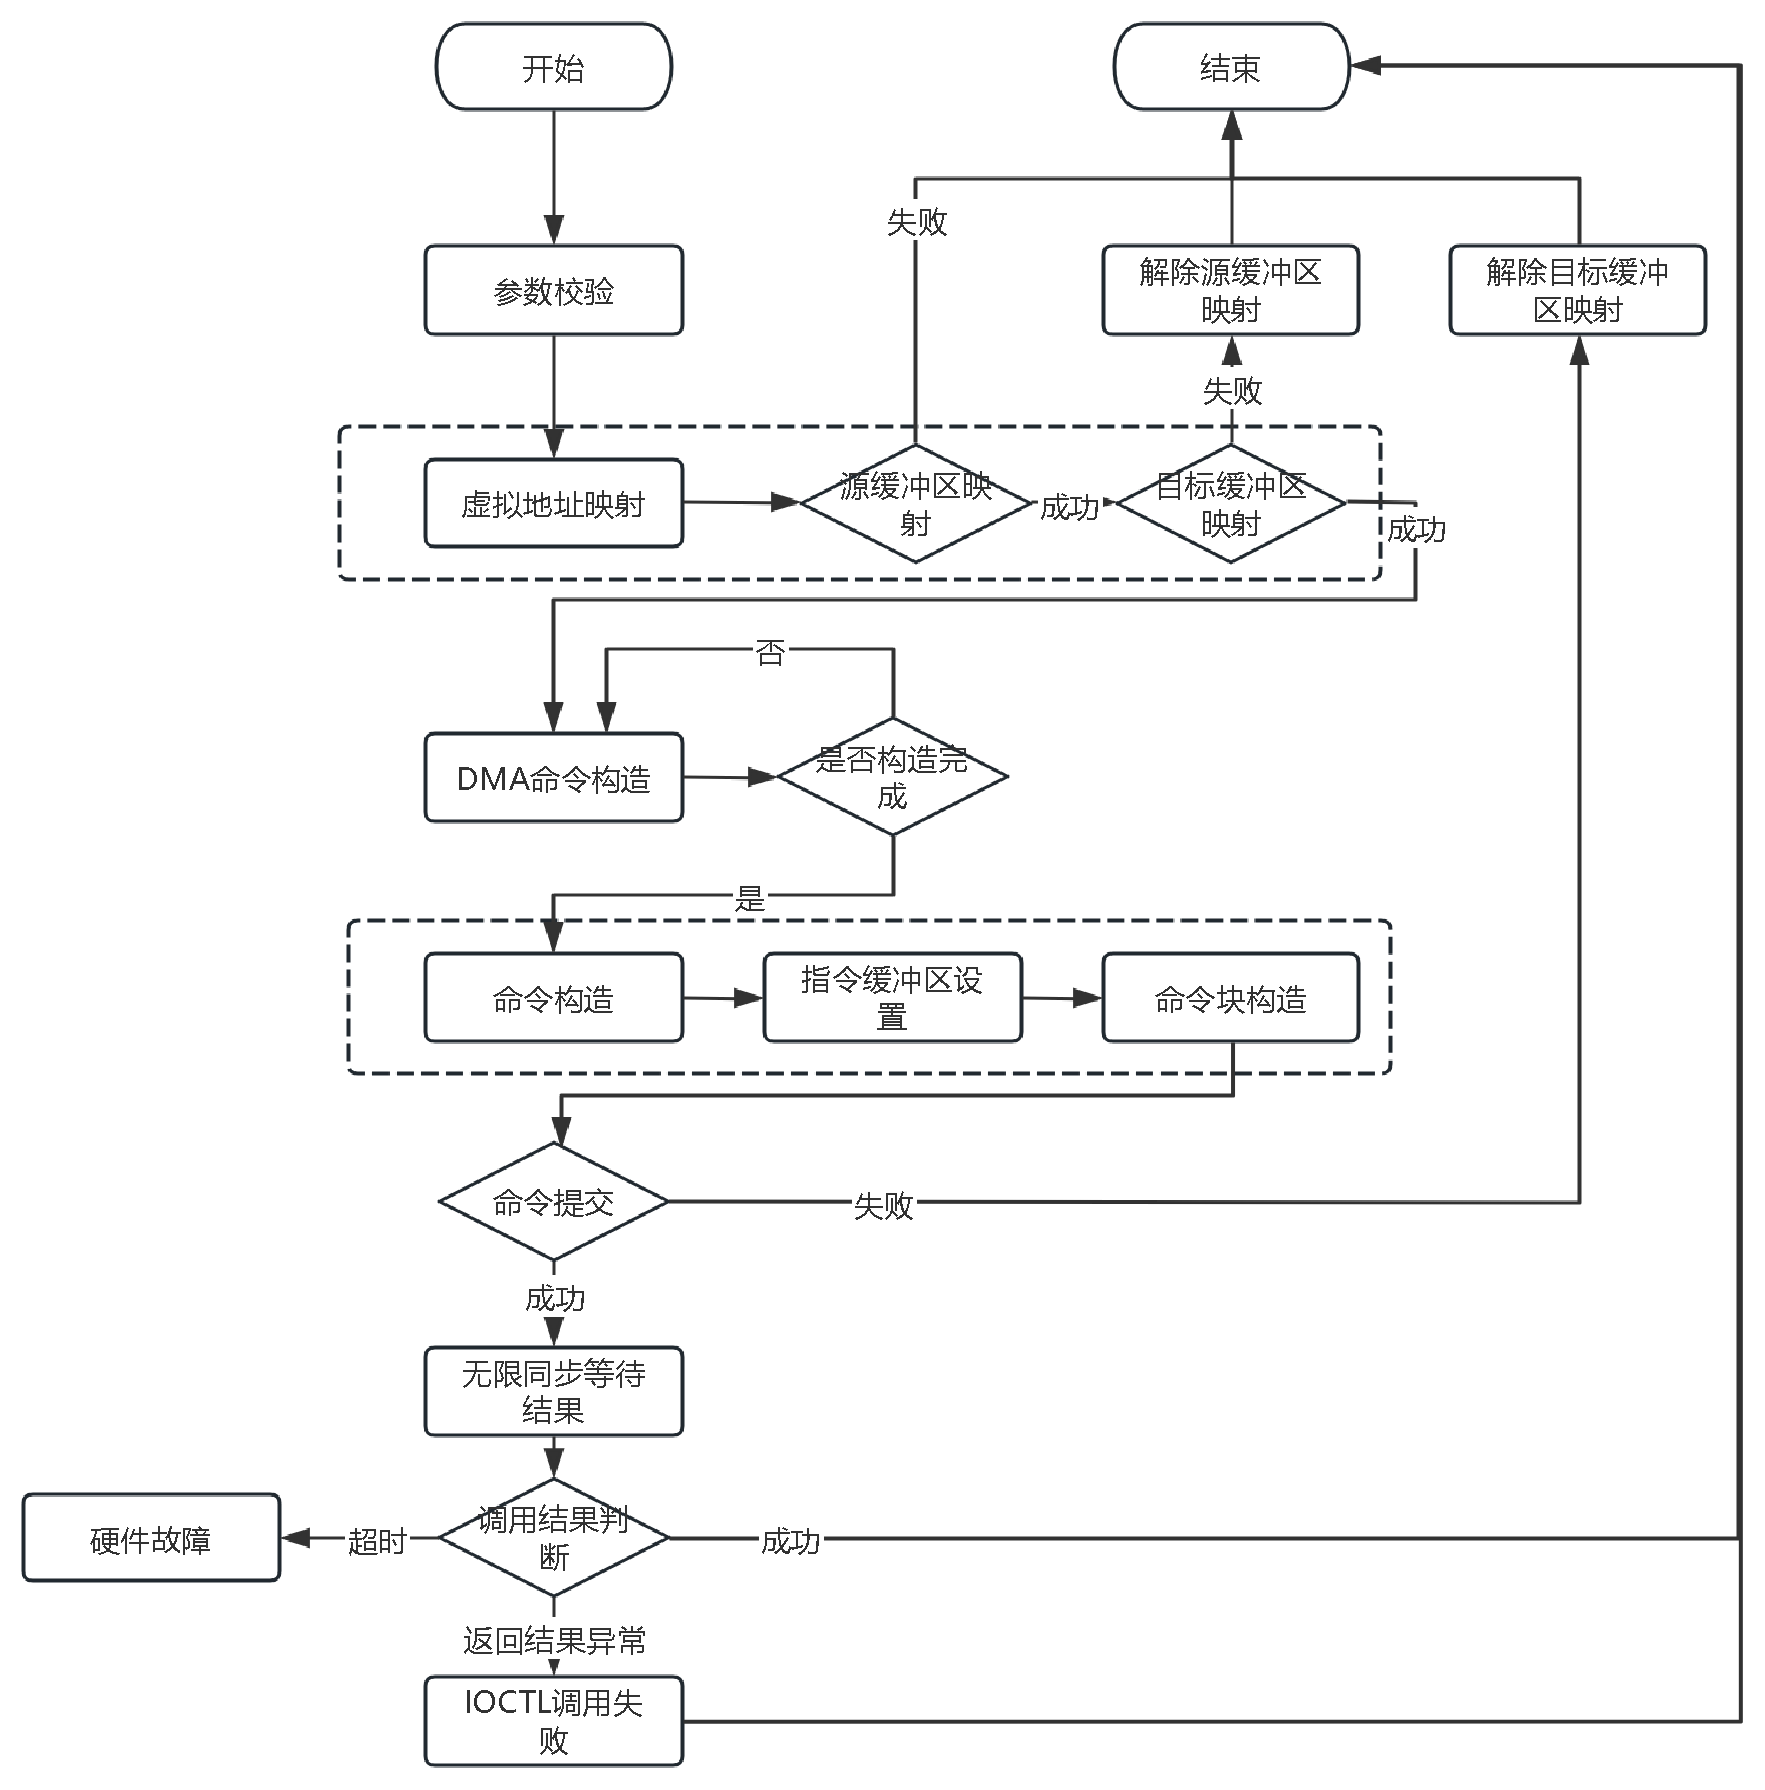
\includegraphics[width=1\textwidth]{lgbm后端-2.pdf}
  \caption{XDMA内存搬运流程}
  \label{fig:lgbm后端-2}
\end{figure}  

\subsubsection{缓冲区对象管理模块}

缓冲区管理模块负责图形缓冲区的创建、导入/导出映射、销毁等,确保显存资源的高效分配与安全释放,是图形栈中连接硬件与上层应用的核心组件。

\textbf{缓冲区创建与销毁}
在使用DRI框架进行缓冲区对象创建时,有使用修饰符和不使用修饰符两种方式。因此有3种创造缓冲区的的方式,创造linear线性缓冲区、使用修饰符创建tile缓冲区以及
使用DRI驱动中的默认创建方式。因此在创建缓冲区时,如果元数据中的tile属性为真,表示创建的是tile格式的缓冲区,在此基础上可以通过判断是否是带有修饰符,
如果带有修饰符,则使用DRI驱动框架中的createImageWithModifiers方法创建缓冲区。createImageWithModifiers 是一个用于创建支持特定内存布局修饰符的图像或缓冲区对象的函数。
而所是元数据中不适用修饰符创建缓冲区则使用createImage创建缓冲区,作用与上一个函数类似。这两种方法在创建时都需要传入宽、高、格式(、修饰符),而格式需要从drm格式转换为dri\_image格式,
在此不过多赘述。而第三种是创建线性缓冲区,需要先初始化缓冲区布局,为图形缓冲区对象计算和设置与格式相关的属性,如步幅(stride)、大小(size)、偏移量(offset)。
步幅是指从缓冲区中某一行的开始位置到下一行开始位置的字节数。换句话说,它是缓冲区内每行数据的跨度,它告诉我们如何从当前行跳到下一行。
偏移量是指从缓冲区的起始位置到某个数据元素的内存地址的距离。大小表示缓冲区所占用的内存空间的大小,通常以字节为单位。
在内存分配参数上选择GTT内存域,并执行GSGPU\_GEM\_CREATE内核调用,创建GTT内存。如图\ref{fig:lgbm后端-3-1}。

缓冲区销毁bo\_destroy是将显卡虚拟空间中的缓冲区对象销毁,将需要销毁的缓冲区对象句柄调用GEM\_CLOSE即可。
缓冲区释放bo\_release是将用户态中的资源释放,但不清除内核态的资源,调用DRI驱动destroyImage方法实现。

步长计算公式:

\begin{equation}
  stride=((width+h\_subsampling-1)/h\_subsampling)*b\_p\_pixel
\end{equation}

步长等与每像素字节数乘以平面宽度与该平面的水平子采样因子向上取整。h\_subsampling是该平面的水平子采样系数,表示该平面的高度相对于原始图像宽度的缩放比例。
b\_p\_pixel表示每个像素的字节数。

\begin{figure}[h]
  \centering
  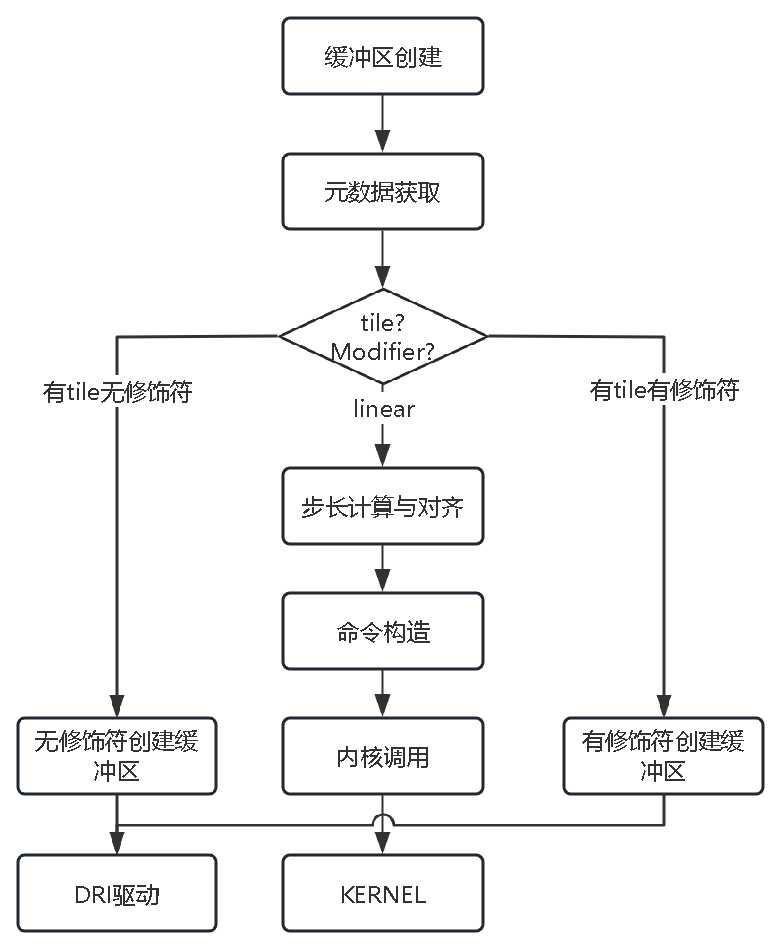
\includegraphics[width=0.6\textwidth]{lgbm后端-3-1.pdf}
  \caption{缓冲区创建流程}
  \label{fig:lgbm后端-3-1}
\end{figure}  

\textbf{缓冲区导入与导出}
缓冲区导入就是从外部缓冲区对象中导入缓冲区,包括获取缓冲区的宽、高、格式、步长等重要属性,是实现缓冲区共享的一个核心功能。
可以使用DRI驱动导入,也可以直接向内核态申请。从流程上需要考虑兼容性,当时用修饰符描述时,可以使用DRI的拓展特性createImageFromFds或者
createImageFromDmaBufs2完成,主要是为了支持一些压缩纹理等特性。也可以调用​DRM PRIME 标准接口​DRM\_IOCTL\_PRIME\_FD\_TO\_HANDLE转换文件描述符为 GEM 句柄。
如图\ref{fig:lgbm后端-3-2}

\begin{figure}[h]
  \centering
  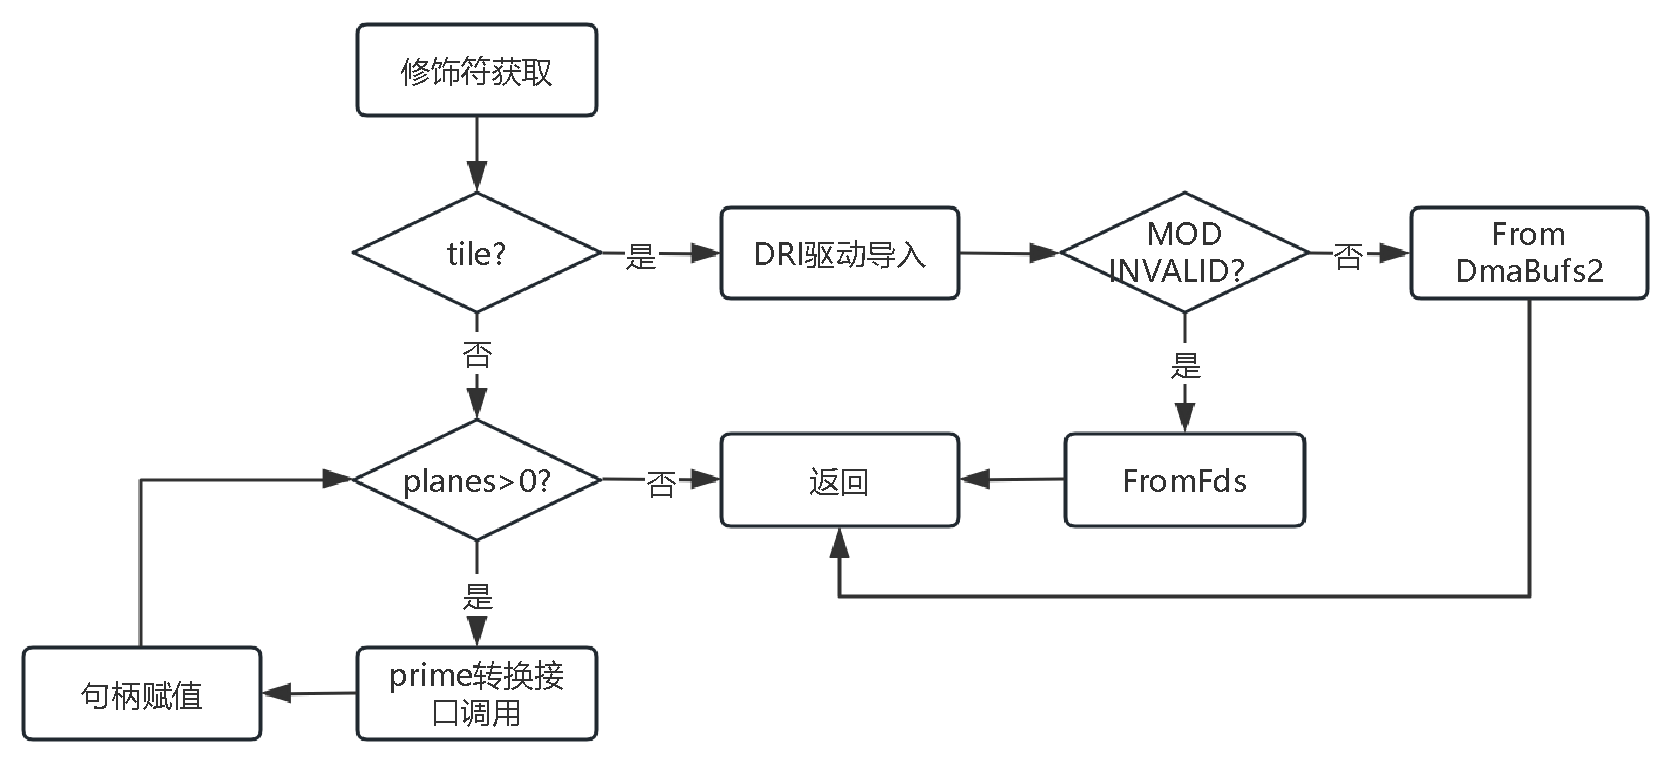
\includegraphics[width=1\textwidth]{lgbm后端-3-2.pdf}
  \caption{缓冲区导入流程}
  \label{fig:lgbm后端-3-2}
\end{figure}  

\subsubsection{内存映射与同步模块}

\textbf{缓冲区映射/解除映射}
%写合并优化
缓冲区映射就是将一个缓冲区从显卡的地址空间映射到系统空间。首先需要通过DRM\_GSGPU\_GEM\_OP命令的GET\_GEM\_CREATE\_INFO向内核查询缓冲区对象的类型,
可能是VRAM或者GTT内存。如果缓冲区对象是VRAM内存,则需要通过XDMA引擎完成从VRAM内存向系统内存的搬运。即先调用GSGPU\_GEM\_CREATE创建一个GTT内存的缓冲区对象,
然后使用前一小节实现的内存传输加速模块功能,实现从源VRAM缓冲区向目标GTT缓冲区的复制。如果缓冲区类型为GTT内存,则不需要进行缓冲区搬运因为此时缓冲区已在系统内存。
但是如果GTT缓冲区标志为写入合并(CPU\_GTT\_USWC),是将多个小写入合并为更大的突发传输,属于CPU优化写入的实现方式。在XDMA引擎正常的情况下,再次申请GTT内存并将
源缓冲区数据写入目标缓冲区。随后使用GSGPU\_GEM\_MMAP获取该GTT缓冲区对象的内核地址,通过mmap将内核地址映射到用户空间,返回用户可访问的虚拟地址。
若任一环节失败则关闭临时创建的 GEM 对象,释放相关内存。
流程如图\ref{fig:lgbm后端-4-1}

\begin{figure}[h]
  \centering
  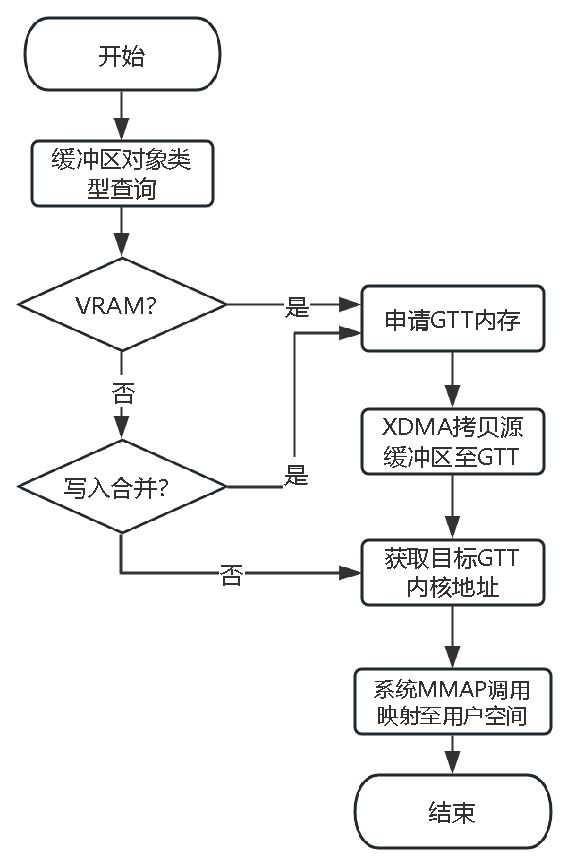
\includegraphics[width=0.5\textwidth]{lgbm后端-4-1.pdf}
  \caption{缓冲区映射流程}
  \label{fig:lgbm后端-4-1}
\end{figure} 

解除缓冲区映射需要先使用munmap系统调用解除用户空间虚拟地址的映射,随后需要根据映射是否需要写回的标志位,判断是否需要将数据从GTT内存写回源缓冲区对象,若是则需要调用XDMA
将修改后的数据写回,写完后使用GEM\_CLOSE关闭临时的GEM对象(即GTT内存的缓冲区对象),如图\ref{fig:lgbm后端-4-2}

\begin{figure}[h]
  \centering
  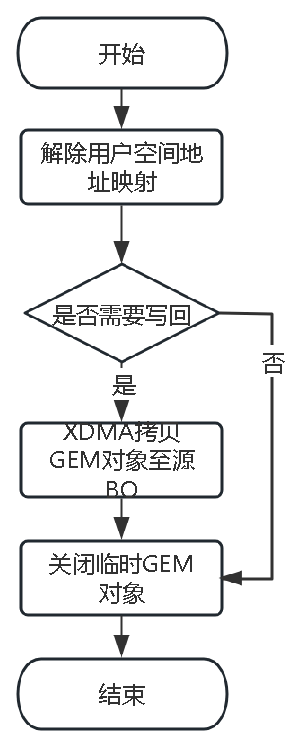
\includegraphics[width=0.5\textwidth]{lgbm后端-4-2.pdf}
  \caption{映射解除流程}
  \label{fig:lgbm后端-4-2}
\end{figure} 

\textbf{缓冲区同步}

缓冲区同步用于确保 GPU对指定BO的操作已完成,以便CPU安全访问或修改BO数据。其核心是通过​等待BO空闲​实现CPU与GPU间的同步,避免数据竞争。
给超时时间设置TIMEOUT\_INFINITE表示一直阻塞到BO空闲或者出错。调用DRM内核的等待指令通知内核等待 BO 空闲,并及时处理一些异常。

\subsection{功能实现模块}
%缓冲区同步,缓冲区复用

本地存储缓冲区和句柄的结构是两个哈希表,一个用于对gralloc\_handle\_t和gralloc\_imported\_handle\_info进行哈希映射,
info包含缓冲区和该句柄引用该缓冲区的数量,用于支持对已注册缓冲区句柄的多次访问支持。另一个对句柄id和缓冲区进行哈希映射以实现快速访问。

\begin{figure}[h]
  \centering
  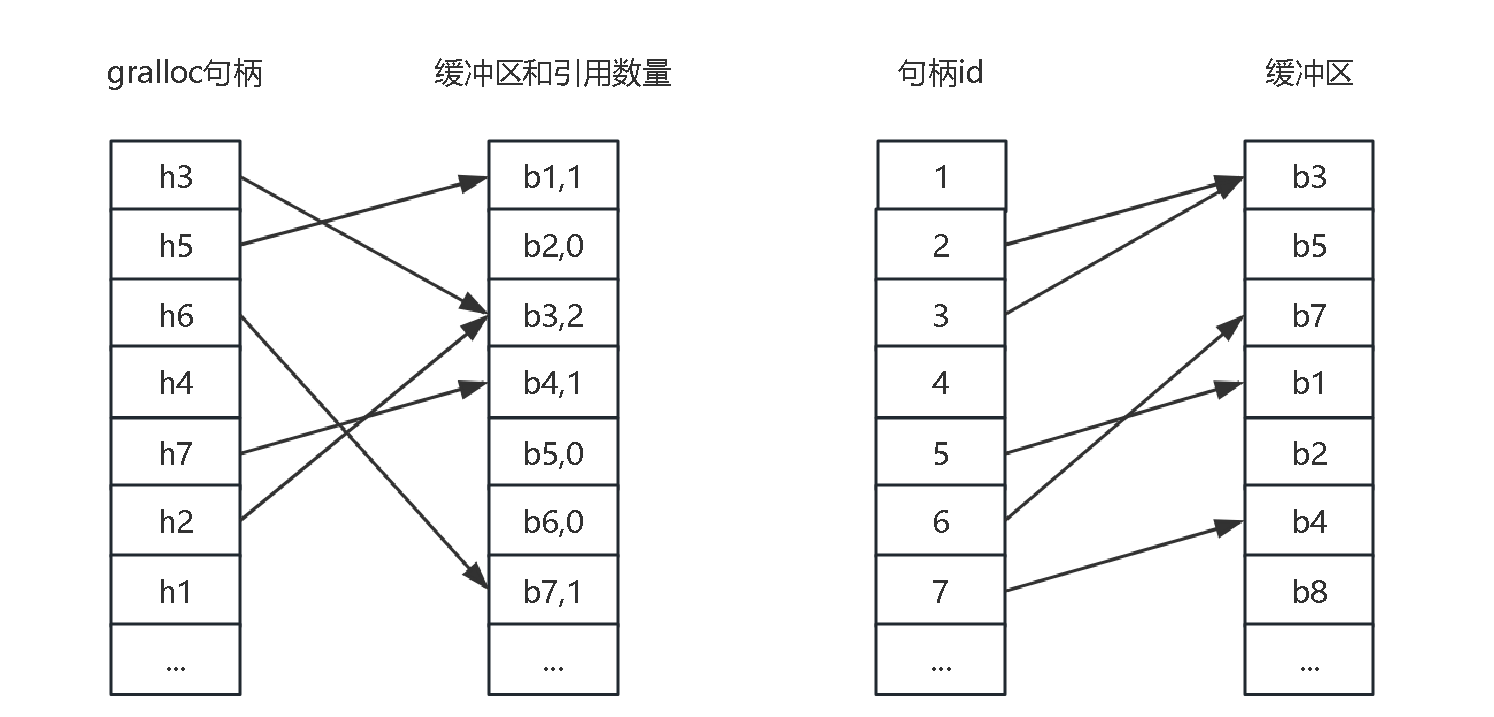
\includegraphics[width=0.8\textwidth]{handle-buffer存储哈希表.pdf}
  \caption{handle-buffer存储哈希表}
  \label{fig:handle-buffer存储哈希表}
\end{figure}

\subsubsection{Allocator模块}
由HAL的设计可知,IAllocator中对于allocate方法的定义为
allocate(BufferDescriptor descriptor, uint32\_t count) generates (Error error, uint32\_t stride, vec<handle> buffers);
该方法根据 BufferDescriptor描述符分配指定数量(count)的图形缓冲区,返回原始句柄数组、行步长(stride)及错误状态,其设计需兼顾 硬件适配性、资源管理 及 跨层级数据传递。
方法中的generates表明需要实现一个异步回调接口,descriptor缓冲区描述符是Mappper模块实现的对缓冲区数据结构的序列化后的二进制字节流,基本类型为
uint8\_t。这是安卓为了跨进程传输所设计,也是因为HIDL接口不支持直接传递复杂结构体(如嵌套对象或动态类型),只能支持基本类型和数组。
count是指需要分配的缓冲区数量,数据类型为uint32\_t。在具体的实现时会重载增加hidlCb参数以实现异步回调的功能。
需要先对gralloc后端驱动进行检查,若未完成初始化,则返回NO\_RESOURCES表示无硬件资源的错误。若驱动已完成初始化,则进行描述符转换,
将HAL层驱动传入的uint8\_t类型的descriptor解码成缓冲区数据结构体BufferDescriptorInfo类型的description。同样,若是接码出现异常则需要
返回BAD\_DESCRIPTOR表示描述符错误。由于上层接口有着count数量的缓冲区进行处理,因此需要初始化一个handle向量用于存储多个句柄。
下面针对单个缓冲区的分配进行描述。接码的description中信息需要转换,convertDescriptor就是是将上层传入的安卓HAL描述符转换成底层通用的描述符。
如安卓的HAL层的DRM\_FORMAT以及缓冲区标志符的命令有所不同,所以需要先进行转换以添加对当前缓冲区格式是否支持的判断。
可以设计出如下的格式转换表\ref{tab:HAL格式转换表}和缓冲区标志转换表\ref{tab:缓冲区标志转换表},此处仅列出一些常用和目前课题硬件支持的格式。

\begin{table}[h]
  \centering
  \caption{HAL格式转换表}
  \label{tab:HAL格式转换表}
  \begin{tabular}{lll}
    \toprule
    HAL\_PIXEL\_FORMAT & DRM\_FORMAT  & value\\
    \midrule
    HAL\_PIXEL\_FORMAT\_RGBA\_8888 & DRM\_FORMAT\_ABGR8888 & 1\\
    HAL\_PIXEL\_FORMAT\_RGBX\_8888 & DRM\_FORMAT\_XBGR8888 & 2\\
    HAL\_PIXEL\_FORMAT\_RGB\_888 & DRM\_FORMAT\_BGR888 & 3\\
    HAL\_PIXEL\_FORMAT\_RGB\_565 & DRM\_FORMAT\_RGB565 & 4\\
    HAL\_PIXEL\_FORMAT\_BGRA\_8888 & DRM\_FORMAT\_ARGB8888 & 5\\
    ... & ...&...\\ 
    \bottomrule
  \end{tabular}
  \note{}
\end{table}

\begin{table}[h]
  \centering
  \caption{缓冲区标志转换表}
  \label{tab:缓冲区标志转换表}
  \begin{tabular}{ll}
    \toprule
    gralloc\_usage & bo\_use\_flags \\
    \midrule
    GRALLOC\_USAGE\_HW\_COMPOSER & BO\_USE\_SCANOUT | BO\_USE\_TEXTURE \\
    GRALLOC\_USAGE\_HW\_FB & BO\_USE\_NONE \\
    GRALLOC\_USAGE\_HW\_RENDER & BO\_USE\_RENDERING \\
    GRALLOC\_USAGE\_HW\_2D & BO\_USE\_RENDERING \\
    GRALLOC\_USAGE\_HW\_TEXTURE & BO\_USE\_TEXTURE \\
    ... & ...\\ 
    \bottomrule
  \end{tabular}
  \note{}
\end{table}

而在此基础上,需要调用驱动的的单个allocate方法,以传入的description缓冲区结构信息实现handle句柄的创建。如果创建失败,则需要释放后端驱动资源以及
回滚已分配的所有handle以保证数据的一致性,主要是使用native\_handle\_close和native\_handle\_delete请除当前句柄的资源,并获取已分配至handles向量中的
所有句柄进行清空缓冲区的操作。若创建成功,则继续初始化元数据Metadata的信息,这个主要是为一些优化方法提供支持。
如果都创建成功则使用handle的setTo方法将创建成功的handle句柄添加至handles向量作为分配缓冲区成功的结果。
而驱动的allocate的算法设计如\ref{algo:GRALLOC_DRIVER::ALLOCATE},主要是使用上一节所述的支持龙芯的gralloc后端方法完成缓冲区的创建,获取宽、高、格式、步长、压缩标志等信息用于
初始化handle句柄并创建gralloc\_buffer等。

\begin{algorithm}
  \caption{GRALLOC\_DRIVER::ALLOCATE}
  \label{algo:GRALLOC_DRIVER::ALLOCATE}
  \SetAlgoLined
  \KwIn{descriptor}
  \KwOut{out\_handle}
  \SetKwProg{Fn}{Function}{}{}
  \Fn{allocate(descriptor, out\_handle)}{
      \tcp{1. 格式解析与对象创建}
      \If{get\_resolved\_format\_and\_use\_flags() 失败}{\Return $-EINVAL$}
      \If{drv\_bo\_create() 失败}{\Return 错误码}
      \tcp{2. 句柄初始化}
      计算 num\_fds/num\_ints\;
      创建 hnd 并初始化 fds 为 -1\;
      \tcp{3. 平面数据填充}
      \For{每个平面}{
          填充 fd/stride/offset/size\;
          \If{失败}{Goto {destroy}}
      }
      \tcp{4. 保留区处理}
      \If{需要保留区 \&\& create\_reserved\_region() 失败}{Goto {destroy}}
      \tcp{5. 元数据与全局管理}
      hnd.id $\leftarrow$ 原子递增\;
      填充其他元数据\;
      \If{创建 buffer 失败}{Goto {destroy}}
      加锁插入全局表\;
      *out\_handle $\leftarrow$ hnd\;
      \Return 0\;
      \tcp{6. 失败逻辑处理}
      Destroy : 
          清理句柄/bo\;
          \Return 错误码\;
  }
  \end{algorithm}

\subsubsection{Mapper模块}
同样,IMapper中的方法有importBuffer、lock、set(实现对元数据的支持)等。其中最重要的方法莫过于导入缓冲区方法importBuffer,
是缓冲区重用的核心方法。该方法定义为importBuffer(handle rawHandle) generates (Error error, pointer buffer);
是将一个原始缓冲区句柄(rawHandle)转换为可在当前进程内安全使用的导入缓冲区句柄。
原始句柄可能来自跨进程传递或克隆操作,直接使用可能存在安全或有效性风险,需通过导入过程生成合法句柄。
同样需要对后端驱动进行检查,流程与allocate方法类似,之后通过getNativeHandle方法获取本地native\_handle\_t句柄,
并且为了确保跨进程的资源独立性,使用native\_handle\_clone复制句柄。
随后使用retain方法从句柄中导入缓冲区对象。若retain失败,需要对复制的句柄调用
native\_handle\_close和native\_handle\_delete关闭并清空资源,并返回NO\_RESOURCES表示无资源错误。
成功则返回导入的缓冲区指针。
retain方法需要先查看当前句柄是否存在于handles\_中,若存在则修改该句柄指向的缓冲区并修改引用计数,返回表示当前句柄已导入缓冲区。
随后查看当前缓冲区哈希表是否存在于buffers\_中(可能被其他进程引用),若有直接修改引用计数,并将新句柄加入handles\_变量即可,没有则需要
导入一个新的缓冲区。算法如\ref{algo:RETAIN}。

% 同时,由于是共享缓冲区设计,所以在导入过程中需要处理一致性等冲突,以及原始句柄的无效性以及错误处理等。

\begin{algorithm}
\caption{GRALLOC\_DRIVER::RETAIN}
\label{algo:RETAIN}
\SetAlgoLined
\KwIn{缓冲区句柄 $handle$}
\KwOut{状态码 (0=成功)}
\BlankLine
加互斥锁 $mutex\_$\;
$hnd \leftarrow$ 转换句柄\;
\If{转换失败}{
    \Return{无效句柄错误}\;
}
\If{handle已注册}{
    增加buffer和handle引用计数\;
    \Return{成功}\;
}
\Else{
    \If{对应buffer存在}{
        增加buffer引用计数\;
    }
    \Else{
        导入新buffer数据\;
        \If{导入失败}{
            \Return{驱动错误}\;
        }
        创建buffer对象并注册\;
    }
    注册新handle和buffer对象\;
    \Return{成功}\;
}
释放互斥锁\;
\end{algorithm}

\subsection{HIDL接口设计与实现}
为了实现绑定式的HAL,需要先根据Android定义的硬件接口规范,使用HIDL语言编写xml文件。编译器会通过该部分的bp文件中定义的vintf\_fragments规则(实际上指向的就是该xml文件),将该
xml文件安装到/vendor/etc/vintf/manifest(系统的安装在/system/etc/vintf/)目录下,在init进程早期阶段通过 VINTF库来加载和解析该目录下的所有HAL实现进行验证并注册。
VINTF 文件中的信息会与设备上已安装的 HAL 实现进行对比以验证 HAL 接口兼容性,在通过 VINTF 文件验证后,Android 会将符合条件的 HAL 接口注册到系统中。
这些接口随后会被 Android 的其他系统服务或应用程序调用。在运行时,VINTF 还负责管理 HAL 接口的动态加载和更新。
通过验证 HAL 接口的版本和兼容性,VINTF 确保系统与硬件设备之间的接口兼容性,避免出现接口不匹配或版本冲突的问题
以Allocator的清单文件为例,使用<manifest>节点作为HIDL文件的起始,
其中version元素的属性表示清单文件的版本号,type表示该清单文件描述的是一个设备类型的 HAL。<hal>节点中的format元素表示该清单描述的是基于 HIDL 的接口,<hal>节点中的
子项name标识了该 HAL 的名称,这是遵循HAL命名空间的约定,表示这是与 Android allocator 相关的 HAL 模块。子项transport表示 HAL 模块使用 hwbinder 作为通信方式。
子项version表示该 HAL 接口的版本号,该版本号为4.0,表示实现的HAL遵循allocator4.0的接口。而<interface>节点中的name元素表示该 HAL 接口的名称是 IAllocator,
是与内存分配器相关的接口,instance元素表示接口的实例名称是 default,通常 HAL 可以有多个实例,但这里指定的是默认实例。而Mapper仅在<transport>子项有所区别,由于Mapper实现的是
直通式,所以是passthrough,且包含arch元素为32+64,表示该接口支持 32 位和 64 位架构。

\section{构建OpenGL ES支持}

龙芯现有的驱动实现基于mesa的gallium架构。
gallium结构可以分为state tracker层,驱动层以及面向操作系统的Winsys层。
state tracker是状态跟踪器,负责将将高级图形API的调用转换为Gallium内部的具体的管道操作。
而驱动层是直接与GPU硬件交互的部分,负责硬件指令生成,就是将Gallium的中间命令转换为GPU特定的指令集;着色器编译,将NIR中间表示编译为GPU原生代码,并进行优化;
资源管理,分配显存、管理纹理和缓冲区对象;命令提交,构建命令缓冲区,并通过winsys提交到硬件队列等。这是硬件特性的最直接体现,它和state tracker组成了
gallium架构下实现OpenGL ES功能的核心组件。而winsys层主要包括显存管理、命令提交与同步、显示输出管理和操作系统平台适配上。
因此在安卓上OpenGL ES实现复用驱动层的实现即可。因此本节仅描述如何构建OpenGL ES支持,并简述目标动态安装库。

龙芯mesa的版本为18.3.6,而由于现有的安卓版本为12.0.0,安卓API版本为31对应的mesa版本为20.3.4,并且由于安卓新的编译方式Soong的加入,
mesa目前最新的版本已经废弃了传统的mk编译方式,转而采用框架外编译的方式。为考虑后续版本的兼容性,因此在现有的mesa18.3.6上采用
mesa原生的ninja编译方式,将生成的动态库文件添加到安卓目标生成目录中。使用安卓框架外编译去生成动态库文件,即用cross-compile配置mesa交叉编译脚本aosp-cross,再使用原生ninja编译规则生成目标安装目录install,
将生成的目标文件安装到AOSP编译框架指定的vendor分区,为后续龙芯mesa版本提供支持。

mesa编译框架如图\ref{fig:mesa编译框架},AOSP编译框架会自动监测所有的Android.mk并编译,Android.mk会调用mesa3d\_cross.mk生成aosp\_cross的mesa交叉编译规则,
按照mesa原生的编译规则生成安装目录install,再将目标动态库文件安装到指定的vendor分区。
\begin{figure}[h]
  \centering
  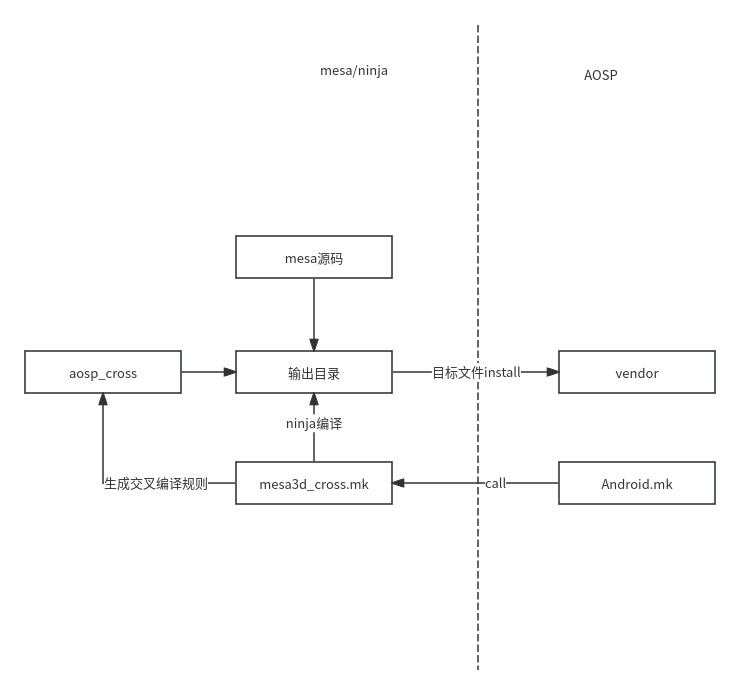
\includegraphics[width=0.8\textwidth]{mesa编译框架.jpg}
  \caption{mesa编译框架}
  \label{fig:mesa编译框架}
\end{figure}

而mesa的目标动态库数据结果如下:

libEGL.so.1.0.0,是一个用于处理 EGL (Embedded-System Graphics Library) 接口的共享库,为 OpenGL ES 或 OpenVG 提供了对底层图形设备的抽象;

libGLESv1\_CM.so.1.1.0,是一个用于实现 OpenGL ES 1.x(特别是 OpenGL ES 1.1 和 OpenGL ES 1.0)功能的共享库),负责将 OpenGL ES 1.x 请求转换为 GPU 可执行的指令;

libGLESv2.so.2.0.0,是一个提供 OpenGL ES 2.x 功能的共享库,用于支持 OpenGL ES 2.x(及以上版本)的图形渲染,提供了着色器的支持等;

libglapi.so.0.0.0,提供 OpenGL API 调用 的代理功能,使得 OpenGL 函数调用可以通过动态链接的方式,调用不同的 OpenGL 实现库;

libgallium\_dri.so,提供了 Gallium 框架下的 Direct Rendering Infrastructure (DRI) 驱动程序实现。

上述数个动态库文件,会被安装到对应的供应商(vendor)分区,以供系统服务调用。而在安卓的命名空间习惯中,由于驱动来源不止mesa项目一种,所以需要将libEGL.so重命名为libGLES\_mesa.so,
以区别不同项目的命名空间。

\section{安卓系统镜像定制}
由于龙芯显卡 LG110 的存储管理单元(Memory Management Unit, MMU)采用页式管理来处理 GPU 所使用的内存,
所有内部功能模块均使用虚拟地址。在连接到内部网络之前,这些地址需要经过转换。当前,MMU 设计了三级页表结构,且页大小(page size)为 16KB。
然而,Android 12 尚未支持 16KB 的页大小。这意味着需要对以下几个方面进行修改:

\textbf{Bionic 库}:需要在 Bionic 中调整页面数据结构,以支持 16KB 的页大小。

\textbf{安卓通用内核文件系统}:在内核的文件系统(如ext4、super和f2fs)中添加对 16KB 页大小的支持。

\textbf{AOSP部分系统服务}:在 AOSP 中的部分系统服务中也需添加相应的支持。

具体实现方法是使用内联函数 page\_size() 来获取内核中的页大小,从而实现对多种页面大小的兼容。这种改动将确保龙芯显卡的 MMU 
能够高效地与 Android 系统和应用程序进行集成,提供更好的性能和兼容性。

% \subsection{内核编译\&bionic\&部分系统服务修改说明}

\subsection{内核定制}
本课题所使用的内核是安卓通用内核5.10,因此在编译时需要添加安卓特性相关的驱动支持如ASHMEM、BINDERFS、BINDERIPC等。
考虑到需要实现对龙芯显卡的支持,在内核编译时需要将loonggpu/lg100\_cp.bin通过CONFIG\_EXTRA\_FIRMWARE选项指定并使用CONFIG\_EXTRA\_FIRMWARE\_DIR指定固件所在的
位置。由于LG110硬件设计上的限制,因此虚拟内存管理只能使用三级页表,页表大小为16Kb。现需要将内核部分模块做硬件适应性修改,如f2fs模块等,
详见表\ref{tab:f2fs模块修改说明}。以此为基础,对f2fs模块中所有依赖这几个宏的相关实现进行修改。

\begin{table}[h]
  \centering
  \caption{f2fs模块修改说明}
  \label{tab:f2fs模块修改说明}
  \begin{tabular}{lll}
    \toprule
    宏名   &   原有  &改动  \\
    \midrule
    F2FS\_MAX\_LOG\_SECTOR\_SIZE & 12 & PAGE\_SHIFT \\
    F2FS\_LOG\_SECTORS\_PER\_BLOCK & 3 & PAGE\_SHIFT - 9 \\
    F2FS\_BLKSIZE & 4096 & PAGE\_SIZE \\
    F2FS\_BLKSIZE\_BITS & 12 & PAGE\_SHIFT \\
    \bottomrule
  \end{tabular}
  \note{}
\end{table}

\subsection{根文件系统定制}
安卓文件系统需要定制的部分可分为bionic和部分系统服务。这两个部分的适配的动机与内核类似,
具体实现可以在bionic/libc/platform/bionic/page.h中实现一个内联page\_size()的函数用以实现从内核
中动态获取页表大小,并以此为适配有使用PAGE\_SIZE为4k相关的服务。这个函数实现是用getauxval来获取与进程相关的辅助值(auxiliary vector values),而
辅助向量是内核传递给程序的额外信息,通常是在程序启动时传递给它的,用于提供关于系统环境的各种信息。AT\_PAGESZ就是辅助向量常量之一,用于查询系统的页面大小,如算法\ref{algo:获取内核页面大小}
同时,由于Android12中有大量的系统服务依然在使用PAGE\_SIZE宏,因此对相关系统服务做一些适应性修改在所难免,共计完成40余处的修改。
\begin{algorithm}
  \SetAlgoLined
  \KwData{void}
  \KwResult{size\_t}
  inline size\_t page\_size(){\\
  \eIf{PAGE\_SIZE已定义}{
    return PAGE\_SIZE\;
  }{
    size = getauxval(AT\_PAGESZ)\\
    return size\;
  }
  }
  \caption{获取内核页面大小}
  \label{algo:获取内核页面大小}
\end{algorithm}

% \begin{figure}
%   \centering
%   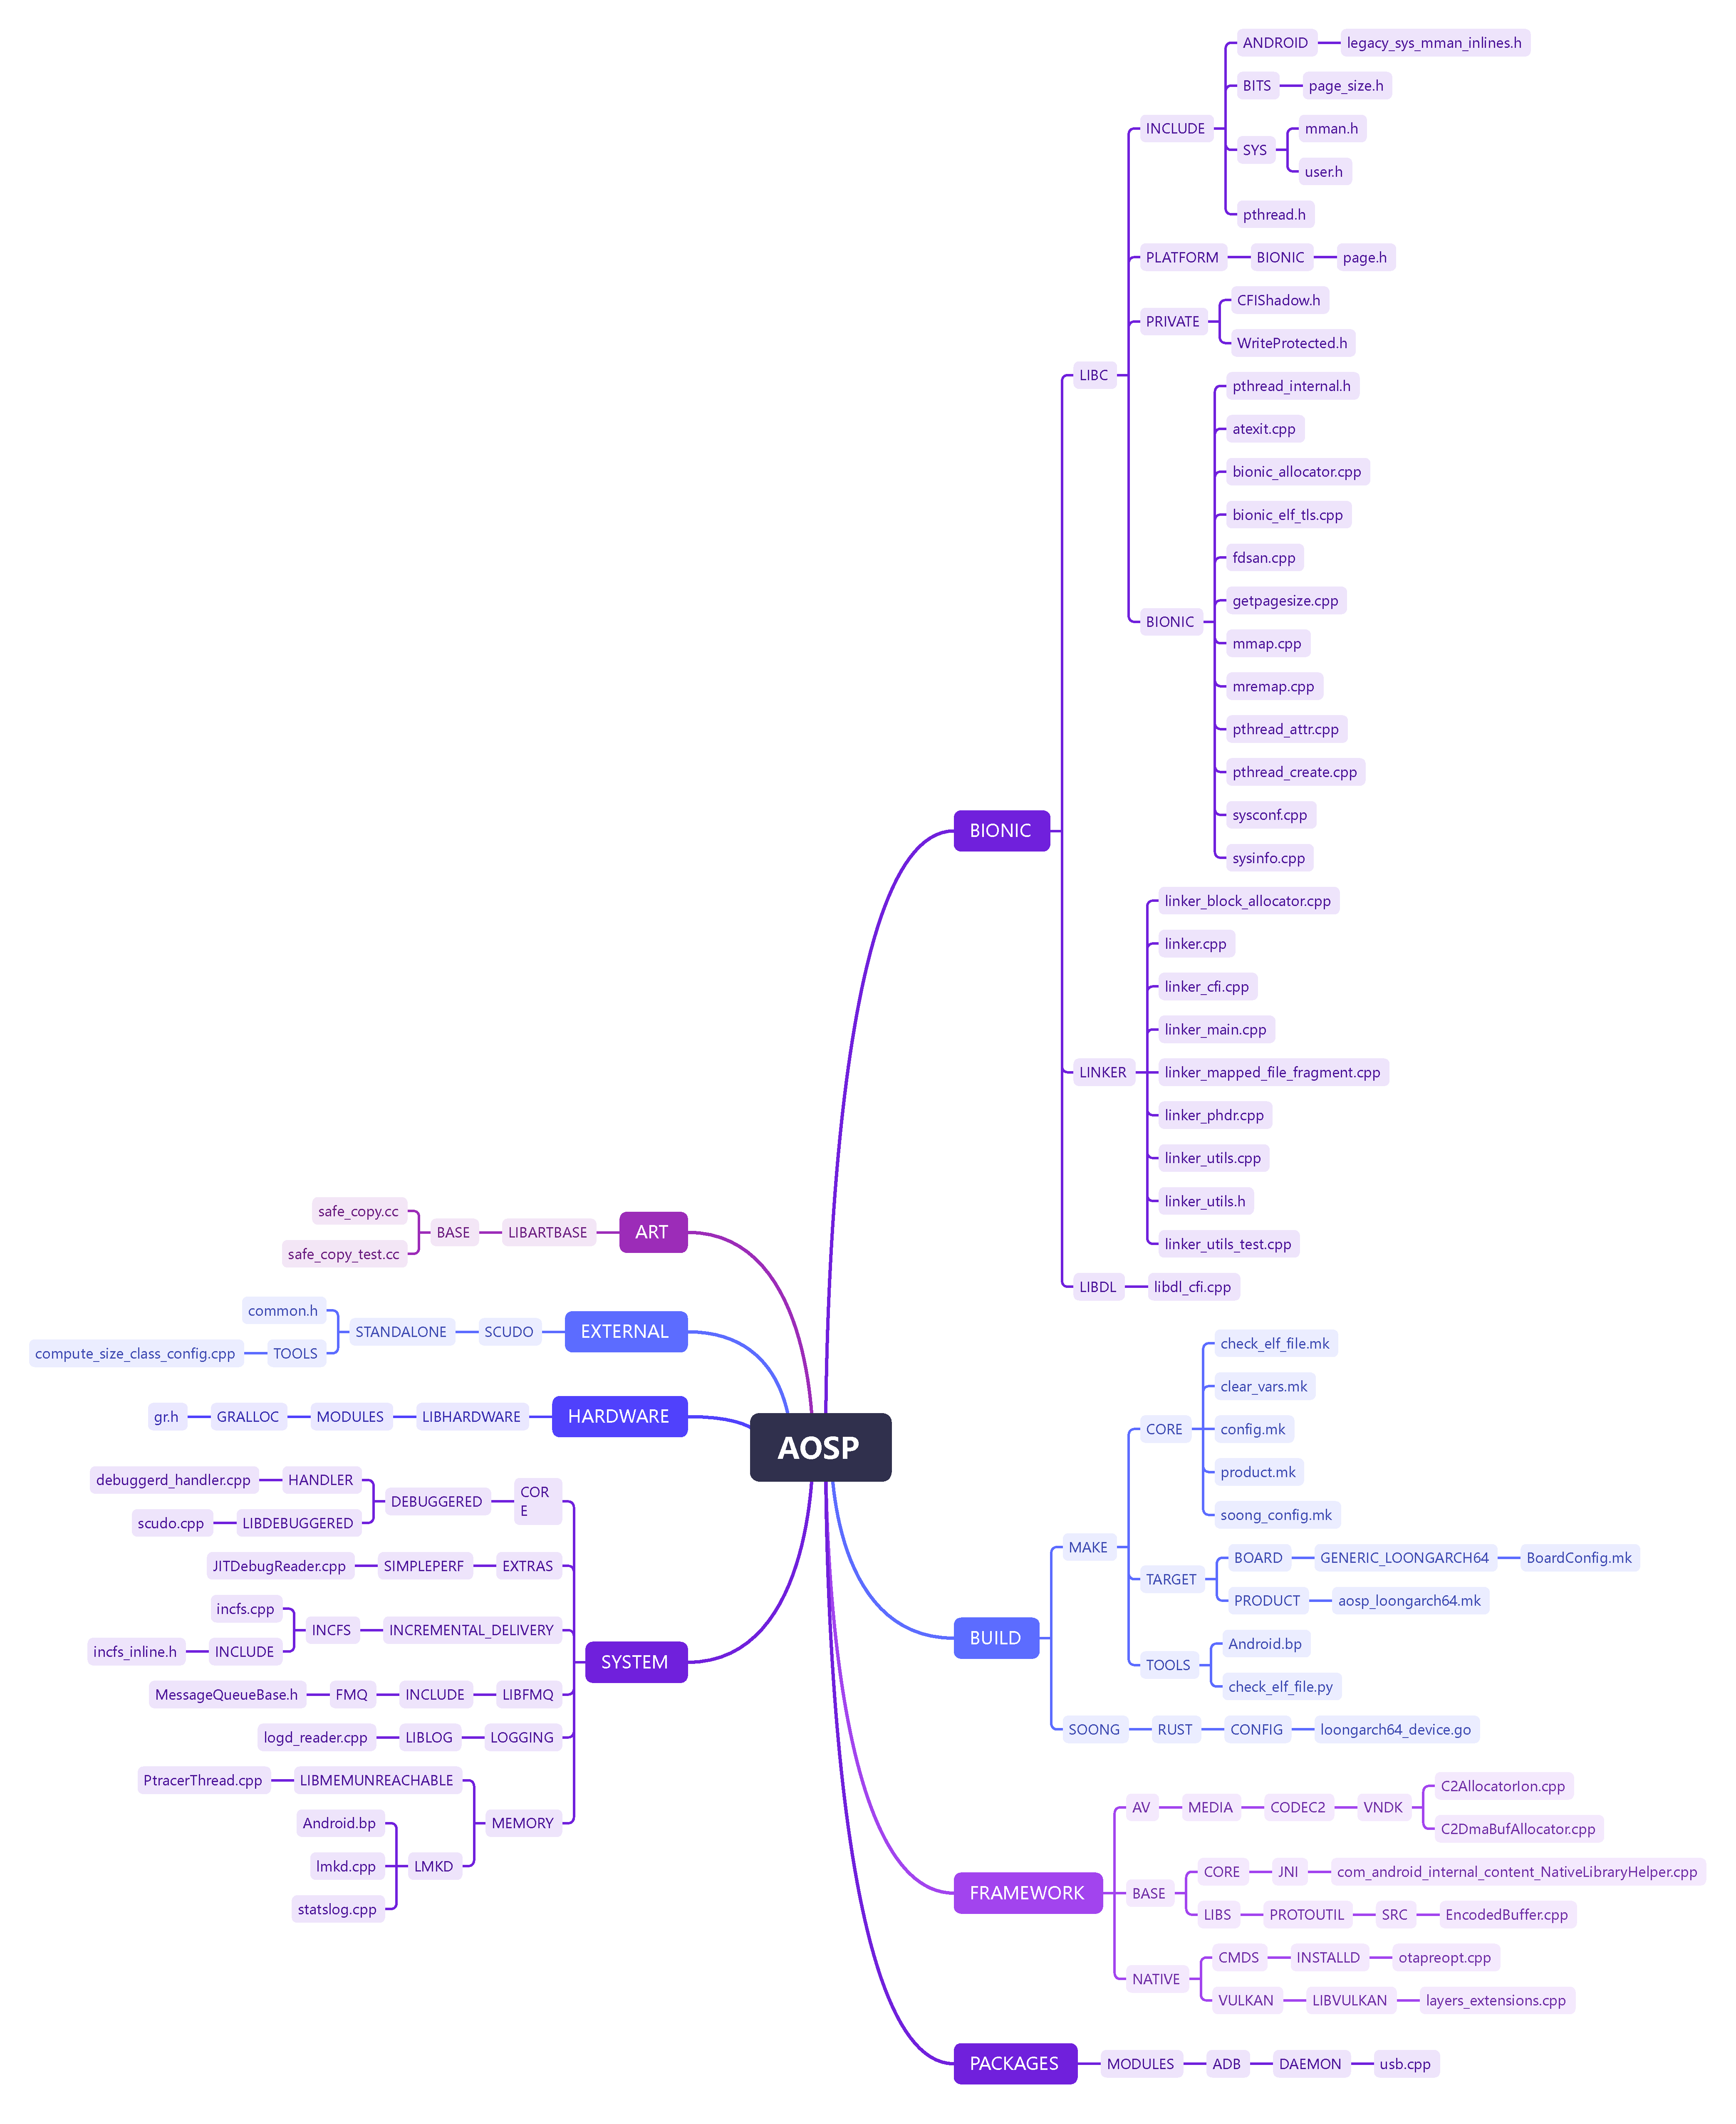
\includegraphics[width=1\textwidth]{androidS+16k适配改动图.pdf}
%   \caption{龙芯androidS 16k适配改动图}
%   \label{fig:androidS 16k适配改动图}
% \end{figure}

\section{本章小结}
本章介绍基于龙芯显卡的安卓图形栈的详细设计和具体实现。说明了三个主要的模块实现:
龙芯GPU内核模块的实现,设计了DRM的ioctl命令码,以及为了适应内核的多版本需求所实现的一套内核驱动模块多版本适配方案;
硬件混合渲染模块简要介绍主要模块功能和具体实现;图形缓存分配模块从硬件支持模块、功能实现模块以及HIDL接口设计与实现这三个部分说明基于LG110的安卓图形缓冲管理HAL层是如何实现的。
然后是说明在安卓上构建OpenGL ES支持的方案,安卓系统镜像定制的方案,以及安卓系统定制镜像方面的设计。

% 字段名	对应的函数	功能描述
% name	"gsgpu_common"	模块的名称,通常用于标识该模块或打印调试信息。
% early_init	gsgpu_common_early_init	早期初始化函数,模块初始化前需要做的一些准备工作。
% late_init	gsgpu_common_late_init	后期初始化函数,在其他初始化完成后执行的工作。
% sw_init	gsgpu_common_sw_init	软件部分的初始化函数,通常用于分配内存、初始化数据结构等。
% sw_fini	gsgpu_common_sw_fini	软件部分的清理函数,用于释放资源、销毁数据结构。
% hw_init	gsgpu_common_hw_init	硬件部分的初始化函数,负责配置硬件寄存器或启动硬件功能。
% hw_fini	gsgpu_common_hw_fini	硬件部分的清理函数,负责关闭硬件功能或恢复硬件状态。
% suspend	gsgpu_common_suspend	挂起函数,通常在系统进入睡眠模式(如 S3)时调用,用于保存硬件状态。
% resume	gsgpu_common_resume	恢复函数,通常在系统从睡眠模式恢复时调用,用于恢复硬件状态。
% is_idle	gsgpu_common_is_idle	判断模块是否处于空闲状态的函数,通常用于调试或节能管理。
% wait_for_idle	gsgpu_common_wait_for_idle	等待模块进入空闲状态的函数,通常用于保证操作完成后再进行后续操作。
% soft_reset	gsgpu_common_soft_reset	软复位函数,用于在某些情况下重置模块,而无需对整个系统进行硬复位。
% \subsection{gralloc}





